%%%%%%%%%%%%%%%%%%%%% chapter.tex %%%%%%%%%%%%%%%%%%%%%%%%%%%%%%%%%
%
% sample chapter
%
% Use this file as a template for your own input.
%
%%%%%%%%%%%%%%%%%%%%%%%% Springer-Verlag %%%%%%%%%%%%%%%%%%%%%%%%%%
%\motto{Use the template \emph{chapter.tex} to style the various elements of your chapter content.}
\chapter{From modern atomism to radioactivity}
\label{Fundamentals-I} % Always give a unique label
% use \chaptermark{}
% to alter or adjust the chapter heading in the running head
\section{Ancient Atomism}

There is a long history of the quest to understand what the fundamental laws of nature are and what things are made of and whether there are fundamental building blocks. In ancient history, these were mostly philosophical questions, but they did spark the curiosity of understanding the how nature fundamentally works, and they did have interesting insights. As a foreword to these lectures we will just very briefly mention the main ideas and philosophers just to give an idea of the times involved. An excellent discussion of the long building of the atomic theory from the ancient atomism to the quantum atom can be found in Ref.~\cite{atomismeantique}\\

The presocratic philosophers in ancient Greece and India were probably the firsts to address these questions nearly three millennia ago.\\
	
%\begin{figure}
%  \centering
%  \includegraphics[width=1.0\textwidth]%{SchoolOfAthens}
%\caption{}  \label{fig:SchoolOfAthens}
%\end{figure}

Thales of Mileto (640-545), the first of the so-called atomists, said ``Water is the first principle of everything''. For Anaximenes (596-595 bc) such unifying unlimited principle must be identified with air.  In his cosmogonic theory, Empedocles (494-434 bc) pretended that
the classic principles are four: earth, water, air, fire.\\

Later on, in ancient Greece, Democritus (470-380 bc) with Leucippus his teacher, the philosophers of the Nature, elaborated the
atomic theory. The question was to know whether matter could be
infinitely divided in smaller parts as believed by presocratics. For the
atomists matter is composed by a very small invisible and
indivisible particle: the atom (meaning indivisible in Greek). Atoms
should be infinite in number, various in shape and moving around in
the void.\\

The atomic view of  matter was however ignored by Plato (428-348
bc) and Aristotles (384-322 bc). Plato tried to describe the
universe in a very imaginative way using five geometrical shapes known
as the Plato's elements. Not long after, Epicurus (341-270 bc) like
Democritus defended the atomic materialist theory believing that
matter is made of indivisible atoms floating in empty space.

\begin{figure}
  \centering
  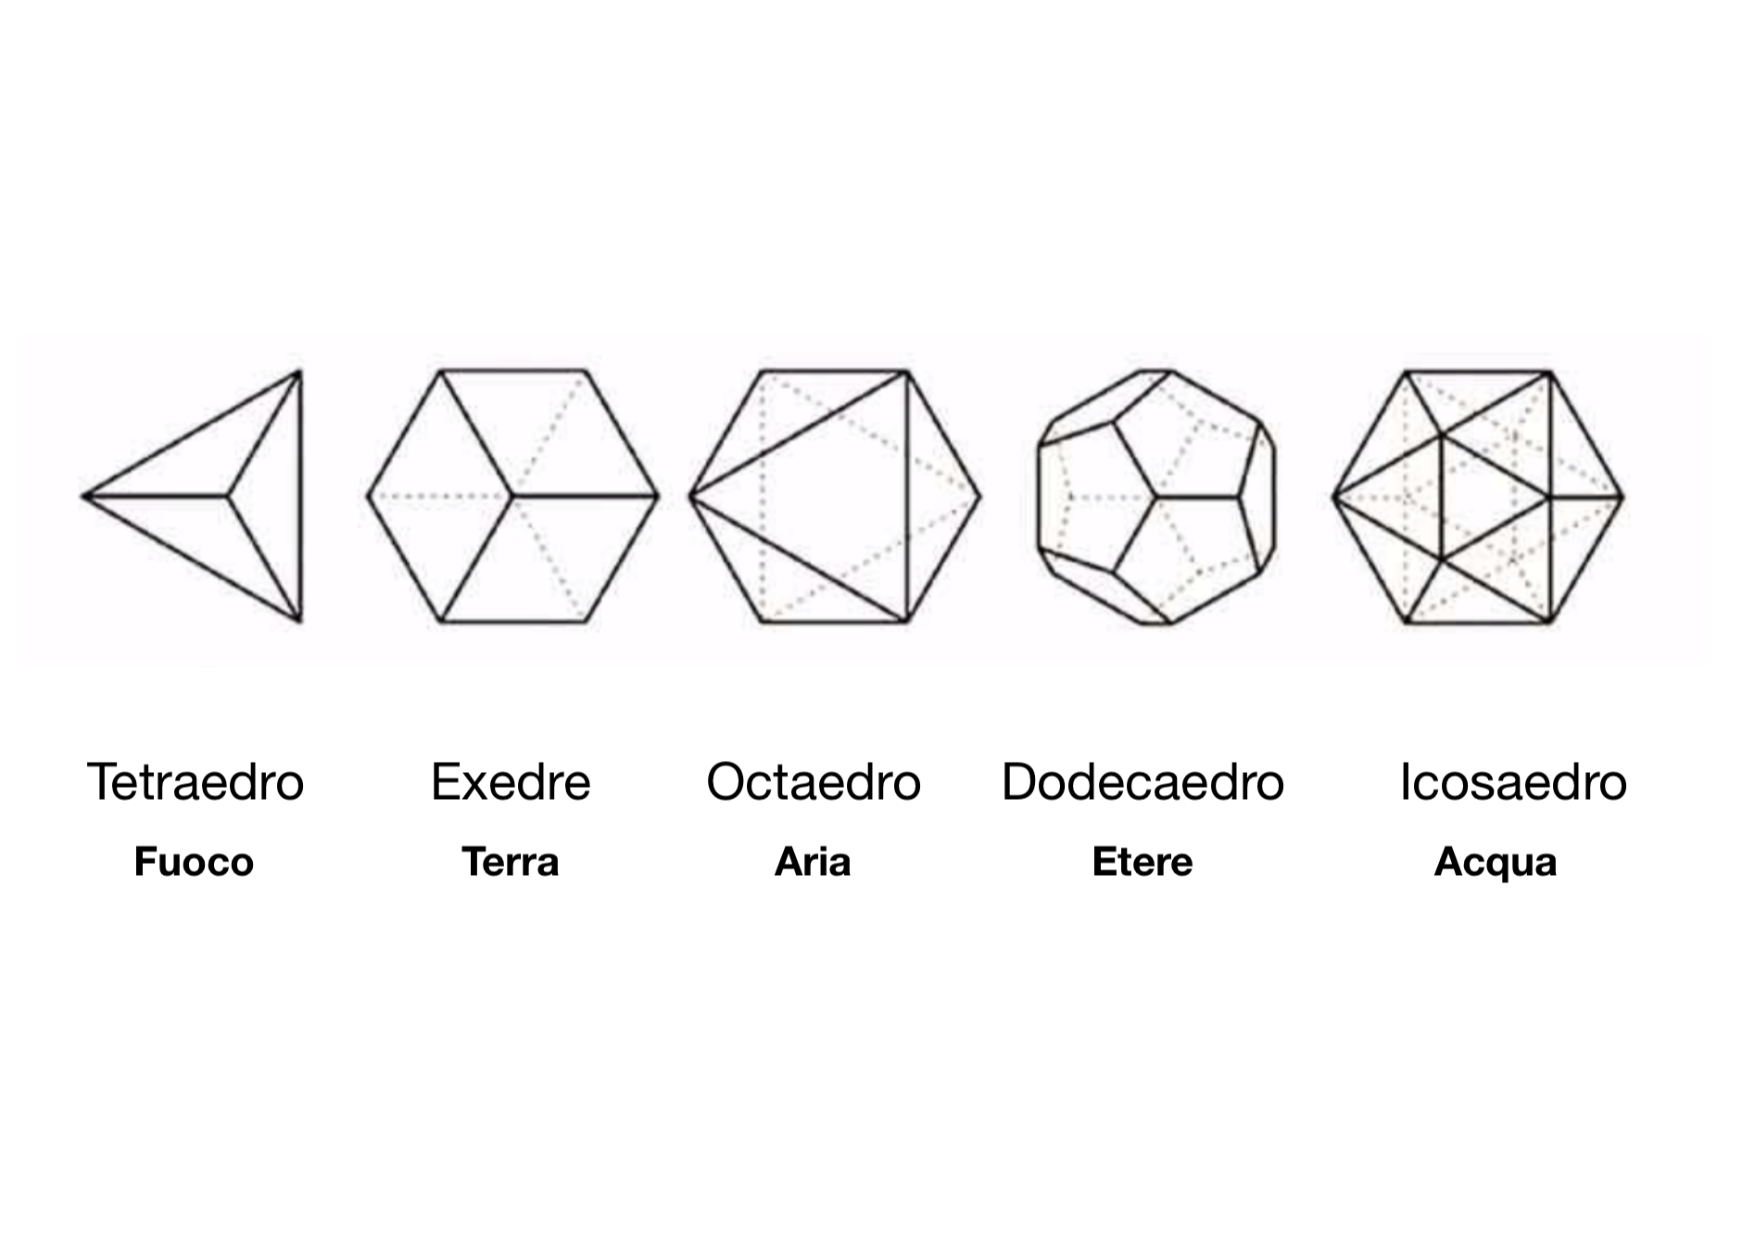
\includegraphics[width=0.8\textwidth]{AncientAtomism}
\caption{The elements from Plato's {\it Timaeus} dialogue, where Plato hypothesized that these regular geometrical forms are the ``classical elements'', i.e. the elements that could explain all complex forms of matter.}  \label{fig:ancientA}
\end{figure}

In Rome, Lucretius (99-55 bc) was the most important nature philosopher and poet, and he was also a definite epicurist. He developed his ideas in six volumes of ``The nature of things'' (\emph{De rerum natur\ae}). He described
the brownian motion of dust particles, taking that as a proof for the existence of atoms. \\

In the ancient Indian philosophy the atomistic theory which appeared
in the VIII century became more elaborated in the I century bc with
the Nyaya naturalists and the Vaisheshikas atomists. \\

The intuitions of the ancient philosophers were remarkable, but at the time they could of course only be philosophical considerations.

\section{Modern Atomism}
\label{Atomism}

The first scientific atomic theory has been proposed in 1803 by John
Dalton. Dalton was an English quacker, a chemist and a meteorologist;
he was color blind and his first paper was on color blindness (which
was called daltonism after him). He also proposed that  matter is made of
blocks of atoms indivisible and indestructible. All atoms of a single
element are identical, whereas atoms of different elements have
different size and mass in order to compose complex structures. 
John Dalton formulated his atomic hypothesis as follows:
\begin{itemize}
    \item matter is made of small particles or atoms;
    \item atoms are indivisible and can neither be created or destructed;
    \item all atoms of an element are identical and have the same mass;
    \item different atoms have different masses;
    \item a compound is made of a fixed number of its constituent atoms (in fixed proportions).
\end{itemize}

It is not completely clear however how John Dalton came to propose his insightful theory. Nevertheless, his theory includes two laws known at the time:

\begin{itemize}

\item The law of mass conservation elaborated and expressed by the
french chemist Lavoisier in 1789, according to which the mass of an
invariant amount of elements remains constant in their chemical
reactions: for example,

		$$ CH_4 + 2O_2 \rightarrow  CO_2 + H_2O.$$

\item The law of definite proportions discovered in 1784 by another French
chemist, Joseph Louis Proust, which states that chemical compounds always combine in constant proportions during chemical reactions  (for example, a fraction of 8/9 -- or to be more explicit 16/18, of the mass of water comes from oxygen and 1/9 from hydrogen).
\end{itemize}

The law of the definite proportions can then be extended to the law of {\it multiple proportions}, stated by John Dalton in 1803, whereby considering two compounds made of two elements A and B (in different proportions), where $r_1, r_2$ are the ratios of the masses of A divided by the masses of B (for each compound $m_A/m_B$), then the ratio $r_1/r_2$ will always be the ratio of small whole numbers. Or in other terms, for any compounds of elements A and B composed by \SI{1}{g} of A, where A is the lightest element between A and B, will require an integer number of grams of B.\\

As an example, let's consider nitrogen (N) and oxygen (O) in the reactions:

$$ 4NO + 2O_2 \rightarrow 4N_2O_3 \; \; {\rm (proportion \; of \; 2:1 \; between} \; 
NO \; {\rm and} {\rm \;O_2)} $$
   
$$ 4NO_2 + 2O_2 \rightarrow 4NO_2  \; \; {\rm (proportion \; of \; 2:1 \; between} \; NO_2 \; {\rm and} \; {\rm O_2 \;)} $$ 

As it is apparent in this example, the possibility that elements could make compounds by themselves such as $O_2$ was not yet taken into
consideration. From the above laws, John Dalton assigned an integer number to elements, by comparison between elements that form compounds. This integer number was referred to as \emph{atomic mass}. In his classification of elements, hydrogen was the lightest and was assigned an atomic mass of 1. Given that hydrogen combines with oxygen in a ratio of masses of 1 to 7, Dalton assigned an {\it atomic mass} of 7 to oxygen, and so on an so forth (see Table~\ref{tab:DaltonElements}). \\

\begin{table}[h]
    \centering
    \begin{tabular}{l c | l c}
    \hline \hline
    Elements & A.M. & Elements & A. M. \\ \hline
    Hydrogen & 1    & Strontian & 46 \\
    Azote  & 5      & Barytes   & 68 \\
    Carbon  & 5     & Iron      & 50 \\
    Oxygen & 7      & Sinc      & 56 \\
    Phosphorous & 9 & Copper    & 56 \\
    Sulphur & 13    & Lead      & 90 \\
    Magnesia & 20   & Silver    & 190 \\
    Lime & 24       & Gold      & 190 \\
    Soda & 28       & Platina   & 190 \\
    Potash & 44     & Mercury   & 167 \\
                 \hline \hline
    \end{tabular}
    \caption{Table of atomic masses (A. M.) of elements according to John Dalton. Azote is the Greek name of nitrogen $\alpha\zeta\omega\tau\iota\kappa o \sigma$ used then by Dalton, and still in use in Italian, French and various other languages.}
    \label{tab:DaltonElements}
\end{table}

This was then resolved in steps. The first was the ideal gas law of Gay-Lussac,:

$$PV = nRT,$$

\noindent where $P$ is the pressure of a gas, $V$ is its volume, $T$ its temperature and $R$ the universal gas constant ($R=8.314$~J/K/mol), and $n$ is the {\it amount of substance} measured in number of moles. Moles are just a unit of number of entities of a substance, defined by the Number of Avogadro (${\mathcal N}_A = 6.02 \times 10^{23}$). This law is known to be correct only in the limit of small densities. This very useful formula in chemistry has actually very far-reaching consequences in the construction of a modern atomic theory. What it is really stating is that in the limit of small densities and at equal pressures, volumes and temperatures, the number of molecules in different gases are equal! \\

This was recognized by Avogadro in 1811 when he proposed that two identical volume of different gas contain the same number of
``particles''. Therefore, in modern terms, the mass has no impact on the volume. Identical volumes of different gas contain the same number of molecules at a given pressure and temperature. As illustrated in figure~\ref{fig:Volumes}, two volumes of $H_2$ are needed for one volume of $O_2$ to make two volumes of $H_2O$. This reaction implies that the oxygen in the initial state has to be forming molecules of two oxygen elements $O_2$. \\
	
\begin{figure}
  \centering
  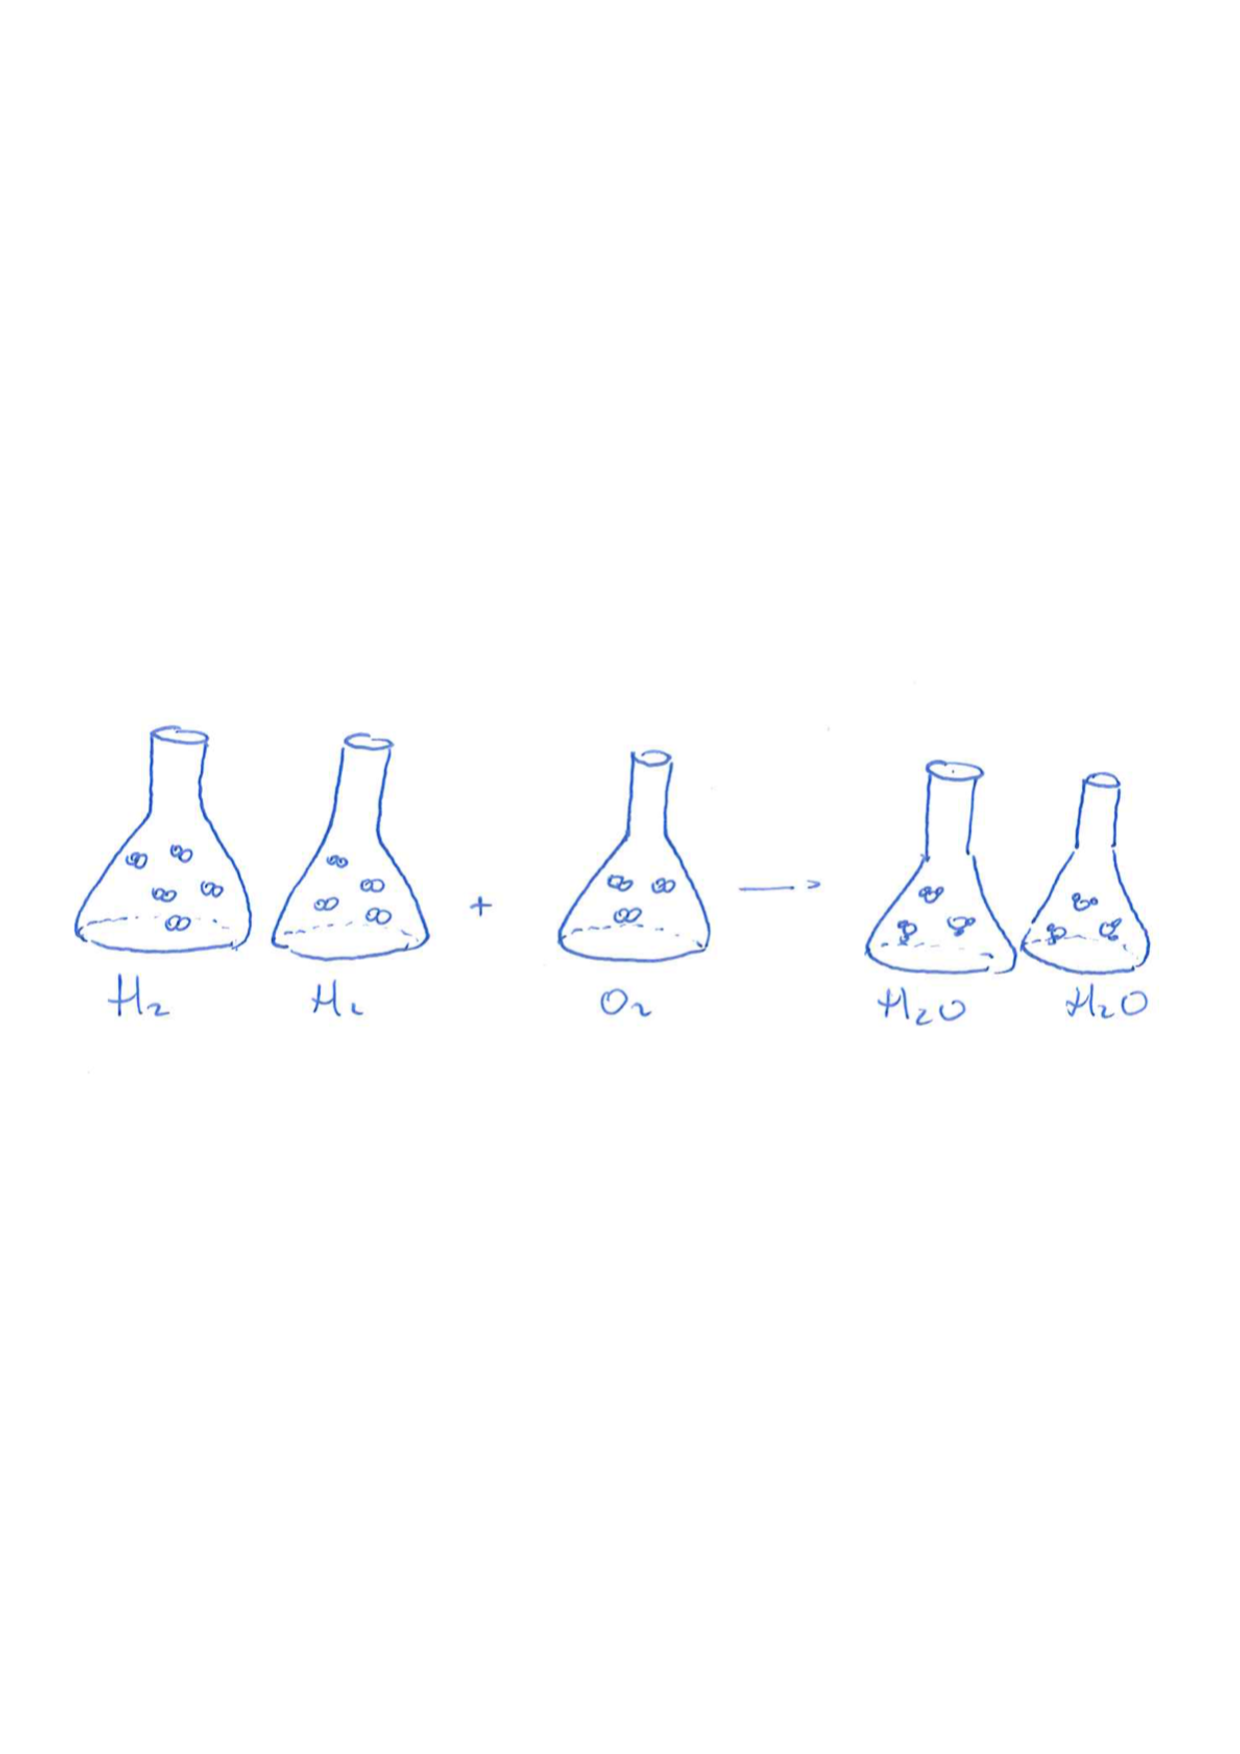
\includegraphics[width=0.8\textwidth]{Volumes}
\caption{Illustration of the implication of the ideal gas law and interpretation by Avogadro that identical volumes of different gases, at given temperature and pressure, contain the same number of entities or ``particles''.}  \label{fig:Volumes}
\end{figure}{}

\section{The proton}
From the laws and the classification in Section~\ref{Atomism}, all elements have  integer atomic masses -- or, in other terms, all elements have masses multiple of the ``first'' element, i.e. hydrogen. In Greek, ``first'' translates to \emph{protos} ($\pi \rho \tau\omicron \sigma$), or \emph{proton}, as the first in the composition of elements. This is a formidable insight in what will then be understood as the structure of the atomic nucleus. \\

\subsection{Atomic mass}
It is interesting to note that while the first element is hydrogen, and was chosen to be the unit of atomic mass by John Dalton, in 1865 the atomic mass unit was chosen to be 1/16$^{\rm th}$ of the oxygen mass, due to the fact that oxygen was very prominently present in a large number of reactions. Current units of {\it atomic mass} are (since 1971) based on Carbon (on its $^{12}C$ isotope, to be precise) due to its very high abundance, high stability and the fact that it has the same number of protons and neutrons (these notions will be more detailed in these lectures). \\

In order to count the number of entities or particles of a substance, at the time the concept of {\it mole} was introduced. It is intrinsically related to the concept of atoms or particles: the idea is to know how many entities are included in one unit of a given element, where that unit is taken to be \SI{12}{g} of $^{12}C$. That is almost equivalent to \SI{1}{g} of hydrogen. \\

To avoid confusion, let's have a brief reminder of some of the related fundamental concepts. If we call $m$ the mass of a sample of a given substance, $m$ is related to the number of entities or particles of the substance, $n$, via its {\it molar mass} $M$, through the relation

$$m = M \cdot n.$$ 

The molar mass, expressed in \si{g/mol}, is the mass of a mole of a given substance. \\

The atomic mass unit, was defined until 2019 to be precisely 1/12 of the mass of a carbon atom. Therefore, until then the mass of \SI{1}{mol} of carbon was precisely equal to \SI{1}{g}. Since 2019, the {\it unified} atomic mass unit was set to be a constant, instead of being fixed to the mass of a given substance:

$$m_u = \SI{1.660539066605e-27}{kg}.$$ % 1.660 \, 539 \, 066 \, 60 \, (5) \times 10^{-27} \; {\rm kg}$$ 

Its numeric value is essentially extremely close to $1/12$ of the mass of a Carbon atom, but it is set as a constant.\\

A simple way to estimate the Avogadro number is taking a given volume of oil (knowing the mass and the nature of the substance) and let it cover a given surface on water. Assuming that the layer is mono-molecular, one can derive the Avogadro number from the measurement of the surface covered by the thin layer of oil. There are of course many more subtle ways to determine the Avogadro number that are beyond the scope of these lectures, the most precise coming from the study of Brownian motion. The current value is:
\begin{equation}
    {\mathcal N}_A = \SI{6.022140857(74)e23}{mol^{-1}}.% 6.022 \, 140 \, 857 \,(74) \times 10^{23} {\rm [mol^{-1}]}
\end{equation}

In this case as well, since 2019 the Avogadro number was fixed to be a constant, precisely:

\begin{equation}
    {\mathcal N}_A = \SI{6.02214076e23}{mol^{-1}}.
\end{equation}

\subsection{The Faraday experiment and the ``charge'' of atoms}

In his insightful electrolysis experiments, in 1830 Michael Faraday published two very important laws on electrolysis that can be summarised in one. \\

\begin{quote}
{\bf Faraday's first law of electrolysis}: the amount of mass deposited on an electrode, due to the flow of current through an electrolyte, is directly proportional to the quantity of electricity that passed through it.
\end{quote}

\noindent The second is a bit more quantitative and also extremely important.

\begin{quote}
{\bf Faraday's second law of electrolysis}: 
when the same quantity of electricity is passed through several electrolytes, the mass of the substances deposited are proportional to their respective equivalent mass.
\end{quote}

\noindent Here the {\it equivalent weight} is the ratio between the mass of the atom and its valence, and the valence is defined as the number of hydrogen atoms with which it can combine. \\

These laws can be illustrated with a simple example: a battery with a Copper Sulfate solution ($CuSO_4$) and two copper electrodes. The observation is that a mass of copper has moved from the anode (+) to the cathode (-). The idea is that, with the electric tension applied between the two copper plates, $Cu^{2+}$ ions are dissolved in water and move towards the cathode. The valence in this case is very important to assess the amount of mass deposited with respect to charge. The valence of copper is $2$. \\

According to these laws, one mole of an element attracted to one of the electrodes will correspond to a definite amount of charges, and in the case of a mono-valent element one has
\begin{equation*} F = 96 485 \; {\rm C/mol},\end{equation*}
i.e. the Faraday constant, which gives the charge corresponding to one mole of element deposited on the electrode. This formula can be generalized to
\begin{equation*}
m = \frac{M q}{F Z},
\end{equation*}
where $Z$ is the electrolyte valence, $M$ the molar mass, $q$ the total charge and $m$ the deposited mass, and $F$ the Faraday constant.

This is very far reaching, since it provides a definition of the unit charge corresponding to a monovalent element, which can be given by:
\begin{equation*}
e = \frac{F}{\mathcal{N}_A} = \SI{1.60e-19}{C},% \times 10^{-19} C
\end{equation*}
which can easily be derived from the simplest system -- the hydrogen atom -- which is monovalent and has a molar mass of approximately $1$. \\

The idea that all atoms could be made of hydrogen was proposed in 1815 by William Proust. The idea emerged that there was a form of unit charge $e$: the concept of \emph{proton}, with unit mass and unit charge, was starting to take shape. However. the discovery of the proton was published in 1919 from the experiment made by Ernest Rutherford two years earlier. This discovery came after the discovery of the existence of the nucleus in 1911, also by Ernest Rutherford.

\begin{framed}
    \begin{experiment}[Discovery of the Proton - Ernest Rutherford, 1919]

Bombarding nitrogen atoms with alpha particles, Ernest Rutherford obtained the following reaction:
		\begin{equation*}\alpha + ^{14}N  \rightarrow  O + p,\end{equation*}
where protons were found to be able to cover long distances.
\end{experiment}

\end{framed}
In the meantime, many other key discoveries which will be discussed in this chapter were made.

\section{Atomic Classification}
A large fraction of the work of the XIX century in Chemistry was devoted to study the physical properties and the reactions of as many substances as possible. A large number of new elements and compounds were discovered. \\

With the massive amount of data and the simple laws stated above, a classification of their properties could be made, according to their atomic masses and their valence. \\

It was the Russian Physicist Dmitri Mendeleev who first started a systematic classification of elements according to their masses and their chemical properties. After a first attempt in 1869, in 1871 he published a classification that highlights the importance of  atomic valence. In his work, valence is reflected in the number of elements with which an element can combine, and can be used to classify the elements according to their electronic valence based on how elements combine with hydrogen and ($H$) and oxygen ($O$). For example, $H$ is mono-valent as it combines with another $H$ to for $H_2$, and therefore $O$ has a valence of II since it combines with two $H$ to form $H_2O$. Elements $El$ that combine with one H to form $ElH$ or with one $O$ to form $El_2O$ have a valence of I. Elements forming $ElO$ or $H_2El$ have a valence of II. Elements forming $El_2O_3$ or $ElH_3$ have a valence of III, and so on and so forth. A classification is shown in Table~\ref{tab:mendeleev}.

\begin{center}
\begin{table}
\begin{tabular}{c cl}
 Valence && Elements \\\hline
 0 && He, Ne, Ar, Kr, Xe, Rn \\
 I &&  H, Li, Na, K, Rb, Cs, Fr, Cu, Ag, Au, F, Cl, Br, I \\
 II && Be, Mg, Ca, Sr, Ba, Ra, Zn, Cd, Pt, Hg, Sn, Pb, O, Se, Te, C \\
 III && B, Al, Au, Fe, Co, Ni, Cr, Mn, Cl, Br, I, Ga, In, Tl, N, P, As, \\ 
 && Sb, Bi, Po \\
 IV && C, Si, Ge, Sn, Pb, S, Se, Te, Pt, Ir, Mn \\
 V && Bi, Sb, As, I, Br, Cl, P \\
 VI && Te, Se, S, Mn, Cr \\
 VII && Mn, Cl, Br, I \\
\end{tabular}
\caption{Classification of elements by Mendeleev, according to their valence.}\label{tab:mendeleev}
\end{table}
\end{center}

Mendeleev soon noticed that elements could be classified according to the number of hydrogen and oxygen elements with which they can combine. In this classification he had eight columns which showed an intriguing {\bf periodicity}, as shown in Table~\ref{tab:FirstPeriodicTable}.

\begin{table}[]
    \centering
    \begin{tabular}{c|c|c|c|c|c|c|c|c}
     \hline  \hline
        \hspace{0.5 cm} & I & II & III & IV & V & VI & VII & VIII \\
         & $El_2O$ & $El O$ & $El_2 O_3$ & $El H_4$ & $El H_3$ & $El H_2$ & $El H$ & $El O_4$ \\  \hline
         \multirow{2}{*}{1} & H & \multicolumn{6}{c}{}  \\
           & 1 & \multicolumn{6}{c}{} \\     \cline{1-8}
         \multirow{2}{*}{2} & Li & Be & B & C & N & O & F & \\
           & 7 & 9.4 & 11 & 12 & 14 & 16 & 19 & \\  \cline{1-8}
         \multirow{2}{*}{3} & Na & Mg & Al & Si & P & S & Cl & \\
           & 23 & 34 & 27.3 & 38 & 31 & 32 & 35.5 & \\     \hline
         \multirow{2}{*}{4} & K & Ca &  & Ti & V & Cr & Mn & Fe, Co, Ni \\
           & 39 & 40 & & 48 & 51 & 52 & 55 & 56, 59, 59 \\     \hline
         \multirow{2}{*}{5} & Cu & Zn & (Ga) &  & As & Se & Br & \\
           & 63 & 65 & 68 & 72 & 78 & 78 & 80 & \\     \hline
         \multirow{2}{*}{6} & Rb & Sr & Yt & Zr & Nb & Mo & & Ru, Rh, Pd \\
           & 85 & 87 & 88 & 90 & 94 & 96 & 100 & 104, 104, 106 \\    \hline 
         \multirow{2}{*}{7} & Ag & Cd & In & Sn & Sb & Te & I & \\
           & 108 & 112 & 113 & 118 & 122 & 125 & 125 & \\     \hline \hline
    \end{tabular}
    \caption{Early Mendeleeev classification of atomic elements (denoted ($El$) according to how they form compounds with hydrogen and oxygen.}
    \label{tab:FirstPeriodicTable}
\end{table}

This first classification starts with a column of alkali metals ($Li$, $Na$, $K$) which have the same valence as hydrogen (these metals have low density and low fusion point). Those appearing in the column VII are the halogens ($F$, $Cl$, $Mn$, $Br$), they easily form compounds with alkalis to form salts (e.g. $NaCl$) and can form bi-atomic gases (e.g. $Cl_2$). Then all elements are ordered according to their atomic masses. This first purely phenomenological classification showed a relation between the atomic mass and chemical properties, and already allowed Dmitri Mendeleev to predict elements in the missing spots in the table. One of them was gallium, which was discovered soon after in 1875 by Lecoq de Boisbadran, and happened to have all the properties predicted by Mendeleeev! This classification also led to introduce the {\bf Atomic Number} which corresponds to the rank of the elements in this periodic table.

Mendeleev's work eventually led to the current grouping in the periodic table of elements, shown in Table \ref{fig:PeriodicChart}. Elements are ordered in terms of their atomic number which is growing by one unit from left to right and top to bottom. The table is further organized in groups of elements with the same valence in columns. It can also be divided in blocks which correspond to the subshell according to the angular momentum $\ell$: the $s (\ell =0)$ subshell corresponds to the two first columns -- including $He$ which has two electrons and completes $1s
^2$, then the elements with their last electrons are in the $p (\ell =1)$ subshell which correspond to the last six columns in the first five rows (excluding $He$), and the elements with their outermost electrons in the $d (\ell =2)$ subshell which corresponds to the 10 middle columns, then the $f (\ell =3)$ is inserted between the $s$ and the $d$ blocs, etc. This classification has been crucial in order to build a quantum theory of the atom. 

\begin{figure}
  \centering
  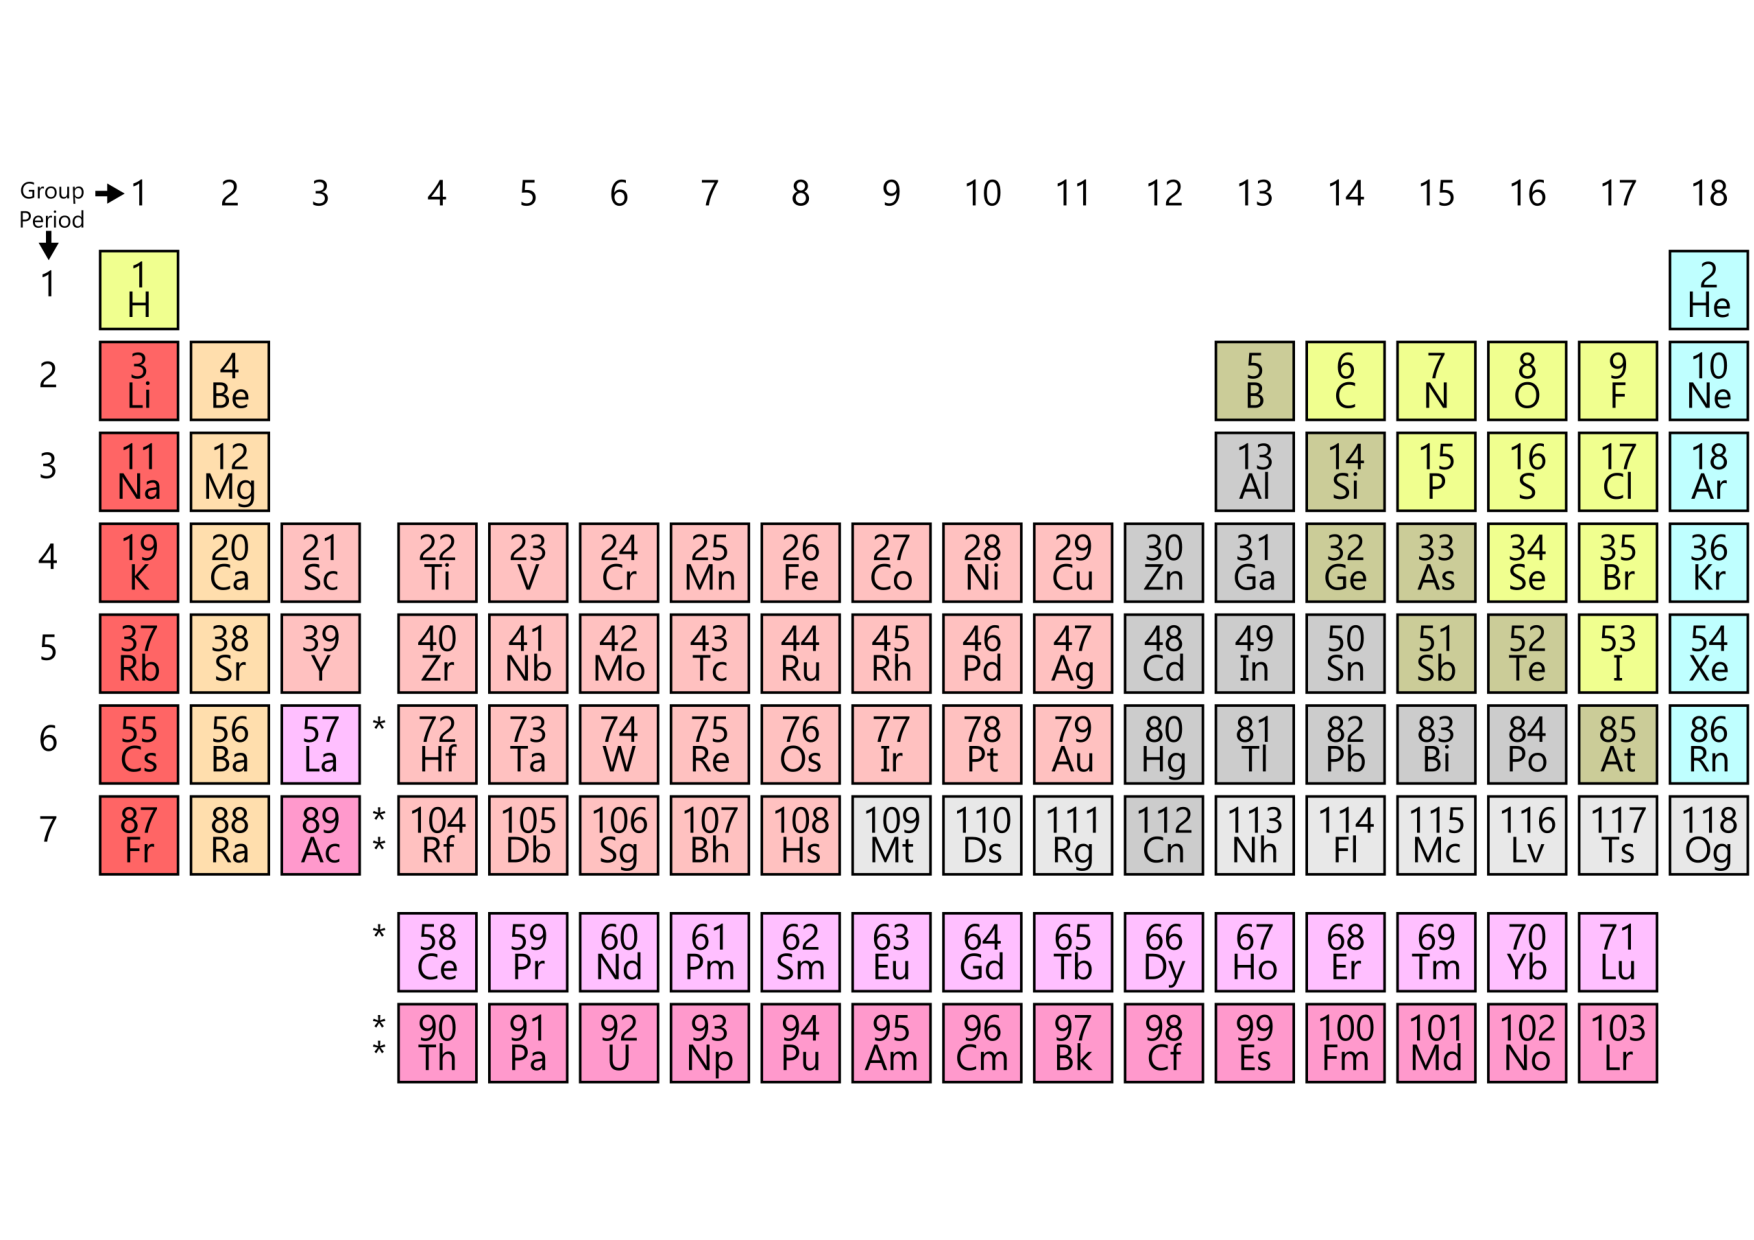
\includegraphics[width=1.0\textwidth]{PeriodicChart}
\caption{Periodic chart of the chemical elements ordered according to their atomic number and electron configuration properties.}  \label{fig:PeriodicChart}
\end{figure}


\section{The Modern Atomic Theory}
In 1827 Robert Brown, a botanist, observed through a microscope that particles of pollen grains of the size of approximately tens of microns in suspension in a fluid, were moving randomly. It was a striking observation that he could not interpret. \\

It was not until 1905 when, in one of his {\it annus mirabilis} papers, Albert Einstein~\cite{BrownianMotion} was able to demonstrate that this motion can be due to the motion of molecules (as for example water molecules in which the pollen particles are suspended), thus demonstrating the existence of atoms. In 1908 Jean Perrin performed a series of measurements that corroborated Einstein's theory stating that it ``cannot leave any doubt of the rigorous exactitude of the formula proposed by Einstein''.

\section{The Discovery of radioactivity}
During the XIX century many discoveries rest on the modern atomic physics and depend on the development of the vacuum tube technologies, namely on the cathode-ray tube. Starting in 1857, Gaissler introduced the glass tube, with two electrodes on each end, to study the electroluminescent discharges. With the help of a vacuum pump he could study the discharge as a function of the gas pressure. Applying high voltage with very low gas pressure, a green luminescence was still obtained on the side of the positive anode. The effect was independent of the presence of residual gas in the tube and of the substances with which the electrodes were made. In 1878 Crookes introduced a fluorescent screen near the anode and demonstrated that the luminescence was associated to the propagation of a kind of ray that could be absorbed by an obstacle generating a shadow on the screen. He could furthermore establish that those cathode rays were deviated by a magnetic field.

\subsection{The discovery of X-rays}
Thomson had not yet described the nature of the cathode rays, when Wilhelm R\"ontgen, a German physicist, on November 8, 1895 discovered that they were producing another type of penetrating radiations invisible to the naked eye depending on the stratification of the material exposed: he gave them the name of X rays. Unlike cathode rays, they could pass through the matter coloring selectively a fluorescent screen or a photographic plate. X rays immediately became widely known because of their ability to visualize bones inside the human body, and R\"ontgen had found this phenomenon experimenting on himself almost by chance. Today we know that cathode rays are electrons, and that X rays are photons irradiated by impinging electrons because of the strong deflection in the atomic nuclei of the anode, which induces bremsstrahlung emission of photons (continuous spectrum), or when the impinging electrons remove electrons from the internal layers, with the release of photons as transition from the external electrons toward the relative gap with energy corresponding to the difference between the two electron levels (striped spectrum). \\
\begin{framed}

\begin{experiment}[Discovery of X-rays - Willhelm R\"ontgen, 1895]

\begin{center}
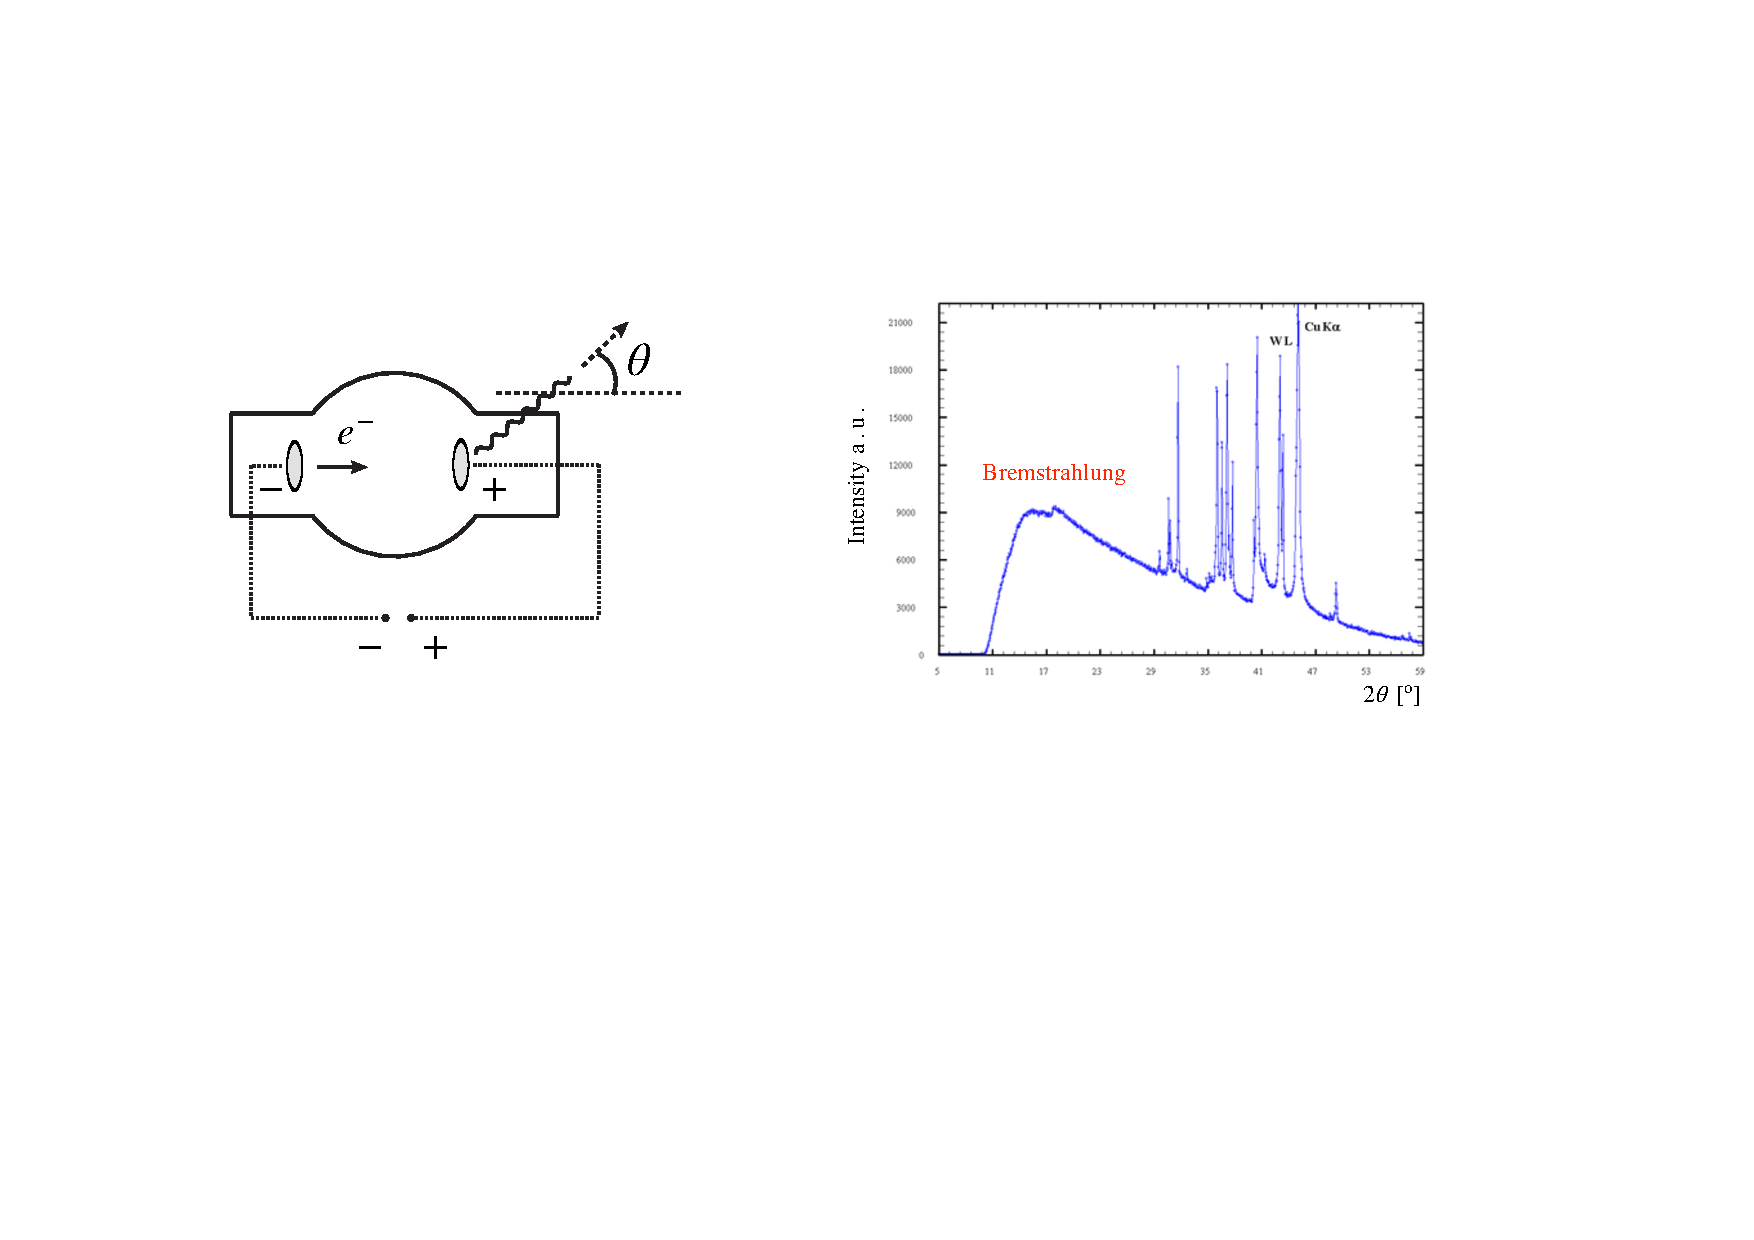
\includegraphics[width=0.95\textwidth]{X-ray-1}
\end{center}

Top: A cathodic tube used by Crooks: the metal Maltese cross was used to demonstrate the cathode ray absorption by the metal of the cross, as it gave a shadow on the fluorescent screen (on the left). This was used as a proof of the fact that cathode rays propagate on a straight line.

Bottom: two examples of X ray production. On the left, the impinging electron kicks off an electron of an inner layer, and a photon is emitted when another electron from the next layer fills the gap. On the right, the photon is instead emitted by the bremsstrahlung of the impinging electron, whose path is deflected by the atomic nucleus.
\begin{center}
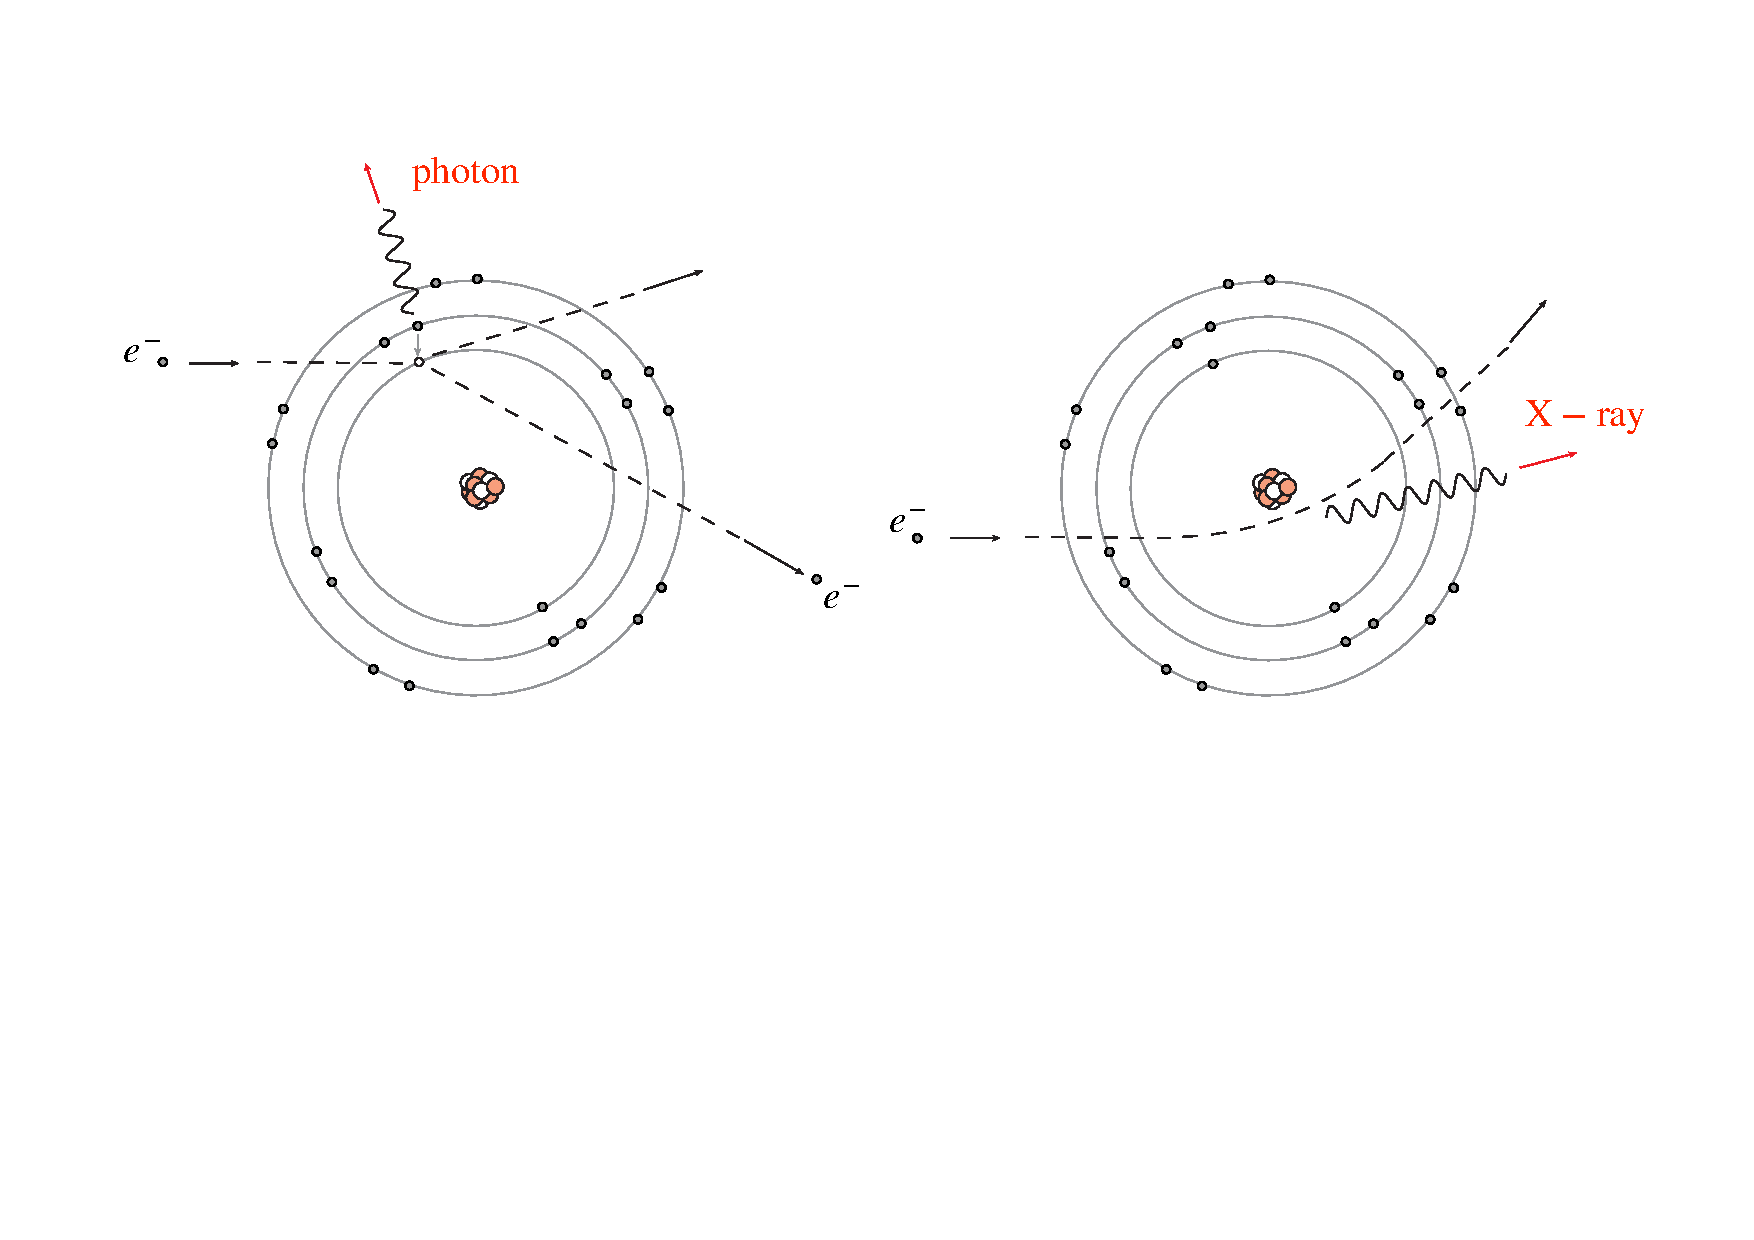
\includegraphics[width=.9\textwidth]{X-ray-2}
\end{center}

\end{experiment}
\end{framed}


\subsection{The discovery of radioactivity and $\alpha$-, $\beta$- and $\gamma$-rays}
\label{sec:DiscoveryRadioactivity}

The intense developments and research in Physics and Chemistry towards the end of the XIX century, led to a ground breaking and completely unexpected discovery. \\

The French physicist Henri Becquerel, who was interested in phosphorescence phenomena, was seeking for a connection between the phosphorescence of uranium salts and possible emission of the recently discovered X-rays. As in the case of phosphorescence, Becquerel was expecting the phenomena to appear after the exposure of the uranium salts to sunlight. \\

\begin{framed}

\begin{experiment}[Discovery of Radioactivity - Henri Becquerel, 1896]


In 1896, Henri Becquerel exposed various salts among which Potassium Uranium Sulfates to sunlight before placing them in front of photographic plates protected from light by black paper. All results failed, except those related to the Potassium Uranium Sulfates. While things were proceeding according to plan, on February 26 -- a cloudy day in Paris (like it's usual in that period of the year) --  Becquerel placed his salts and photographic plates in a closet. On March 1, by scientific rigor, Becquerel decided to develop the photographic plates. Much to his surprise, the images were clearly impressed and even even the shape of a copper cross which had been placed by chance between the salts and the plate was impressed. Becquerel had discovered natural and spontaneous radioactivity (the term \emph{radioactivity} was given by Maria Sklodowska-Curie). The conclusion was that the material was spontaneously emitting radiation which had properties similar to X rays.
\end{experiment}
\end{framed}

In 1898 Maria Sklodowska-Curie, in collaboration with her husband Pierre Curie, working on an uranium mineral extracted from uranite (or pitchblende), demonstrated that a radioactivity much more intense than the one due to the uranium salts was associated to two chemical elements not known until then, which they called polonium and radium. \\

The same year Ernest Rutherford demonstrated that natural radioactivity observed at that time was due to radiation different from X rays. To further study the nature of these spontaneously-emitted radioactive rays, Rutherford built a device which used led to collimate the rays and study their behaviour under magnetic field (see Fig.~\ref{fig:Radioactivity}).  \\

\begin{figure}
    \centering
      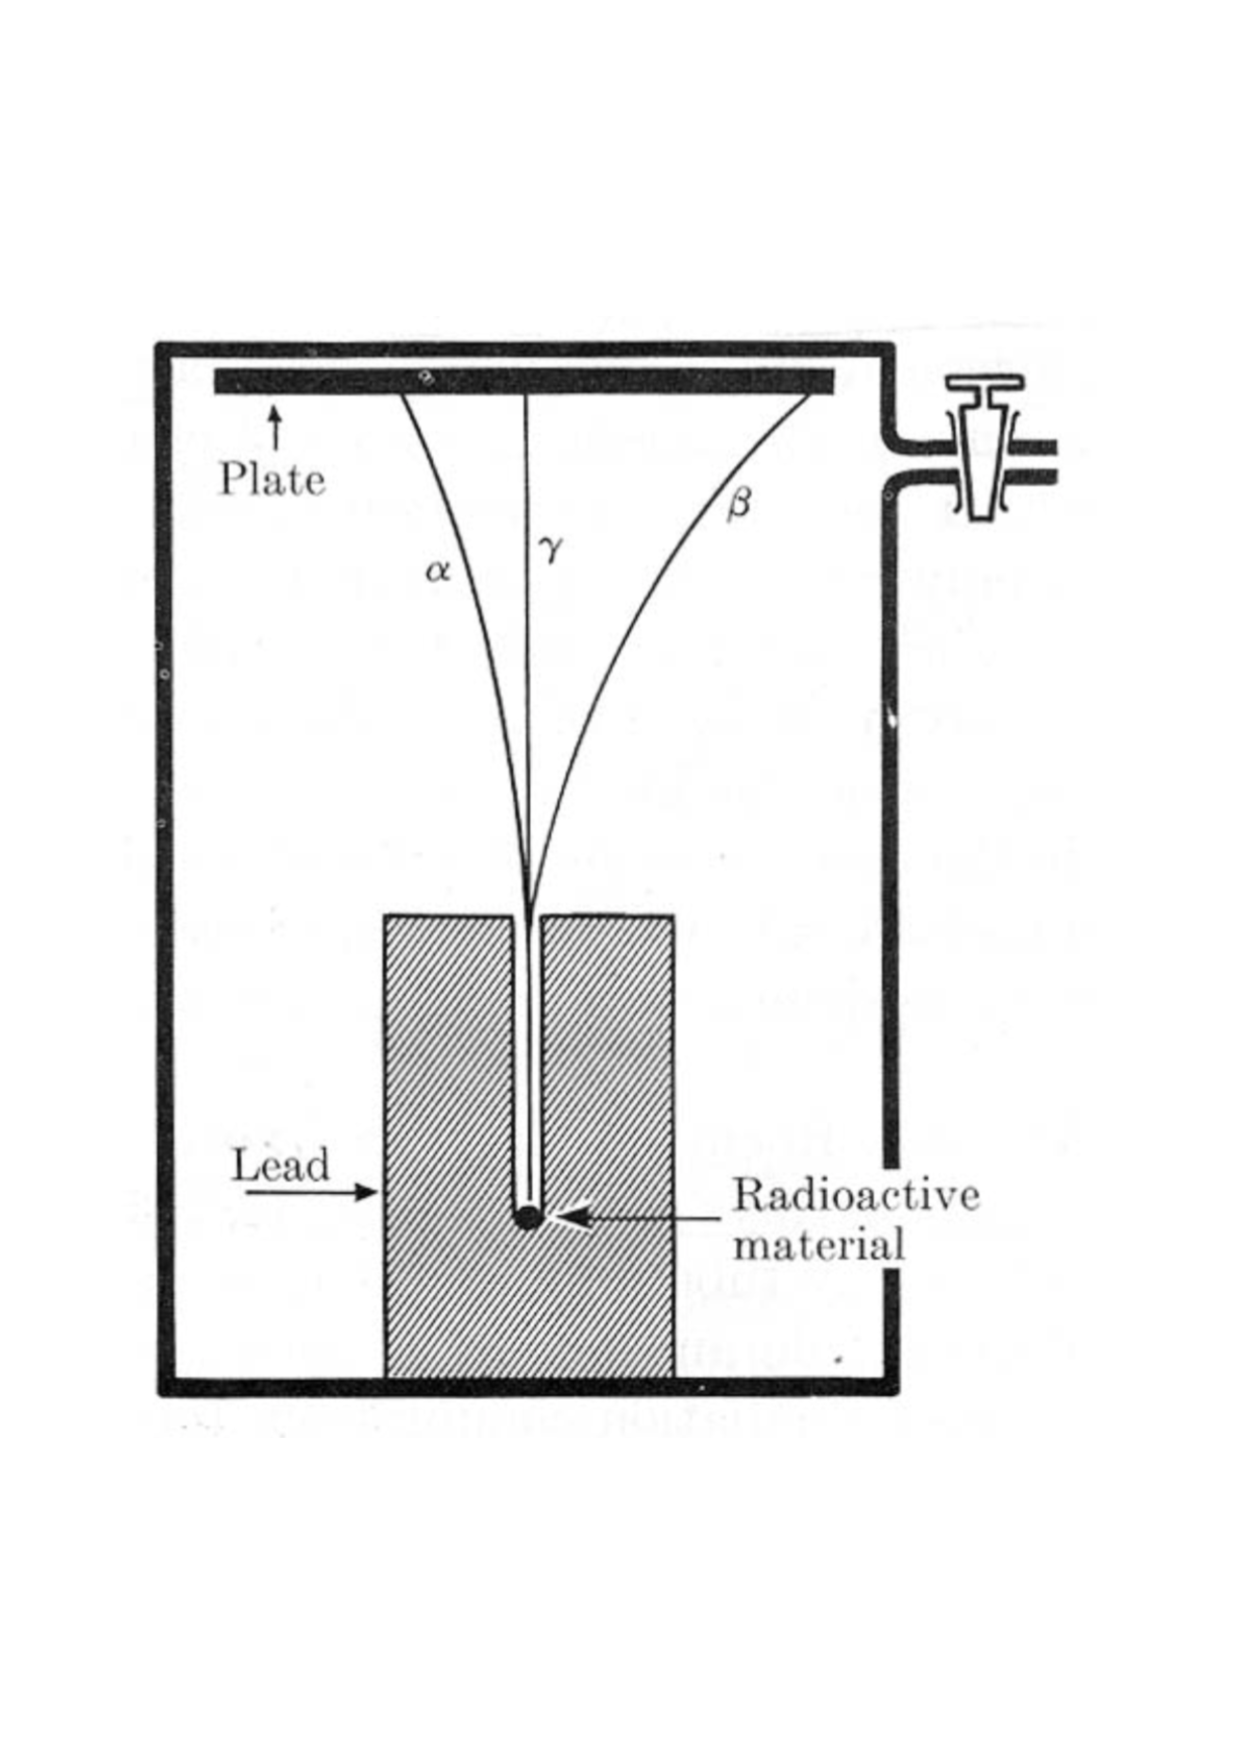
\includegraphics[width=.4\textwidth]{Becquerel}
    \caption{The device used by Ernest Rutherford.}
    \label{fig:Radioactivity}
\end{figure}

Different radioactive substances were placed in the device and the rays were either deflected in different directions or were not deflected. This showed that there were three types of radioactivity: one negatively charged, one positively charged and one neutral. The non-deflected neutral component was discovered in 1900, by the French physicist Paul Ulrich Villard. \\

By placing different absorbing materials in the path of radioactive rays, the different types of radiation could be characterized in terms of their penetrating power. The deflected types of radiations were named $\alpha$ and $\beta$, which were deviated in opposite directions by an external magnetic field. The neutral radiation was called $\gamma$. \\

In 1900, Becquerel verified that the ratio $e/m$ of the cathode rays experiment (described in Sec.~\ref{sec:ElectronDiscovery}) and that of the $\beta$ rays were identical: $\beta$ rays therefore seemed to be electrons. \\

In 1909, Rutherford identified the $\alpha$ rays as nuclei having a charge of $2e$, which were subsequently understood to be Helium $^4{\rm He}^{2+}$ ions. \\

\begin{table}[]
    \centering
    \begin{tabular}{llllll}
    \hline \hline
    Radiation    &  Nature  & mass & Energies & Spectrum & Penetration \\ \hline
    $\alpha$ & Helium ($^4{\rm He}^{2+}$) & 3.73~GeV & few MeV & Discrete & 6-7~cm \\ \hline
    $\beta-$ & Electron ($e^{-}$) & 0.511~MeV & from keV to MeV & Continuous & 5-7~m \\ \hline
        $\beta+$ & Positron ($e^{+}$) & 0.511~MeV& from keV to MeV & Discrete & 5-7~m \\ \hline
    $\gamma$ & Photon ($\gamma$) & 0 & from keV to MeV & Discrete & $\sim$~km \\ \hline
       $X$ & Photon ($\gamma$) & 0 & from $\sim$100~eV to keV & Discrete &  $\sim$~km \\ \hline \hline
    \end{tabular}
    \caption{Properties of the main forms of radiation: nature, mass, ranges of energies and penetration lengths.}
    \label{tab:Radioactivity}
\end{table}

\section{The discovery of the electron}
\label{sec:ElectronDiscovery}

It is interesting to note that while Crooks' tube was succesfully used to discover X rays, the nature of the initial beam was not fully known. The presence of something flowing from the cathode towards the anode in Crooks' tubes was known since 1876. This was understood by Eugene Goldstein who named them \emph{cathode rays}. The characterization of these rays came later from the development of cathode rays tubes (CRTs\footnote{The same technology used to build monitors and televisions until 2000s.}), which are vacuum tubes (as opposed to Crooks tubes, which were filled with tiny amounts of air).\\

It is in 1897 that Joseph John Thomson studied and discovered the nature of these electric charges. \\

\begin{framed}
\begin{experiment}[Discovery of the Electron - Joseph Thomson, 1897]
    
    The experiment conceived by Joseph Thomson used a cathode ray tube. The source of electrons can be simply a cathode, or they can be produced from a heated filament or from exposure to radiation. There is then an accelerating gradient to accelerate the cathode rays along the longitudinal ($x$) direction, see the Figure below:
    
        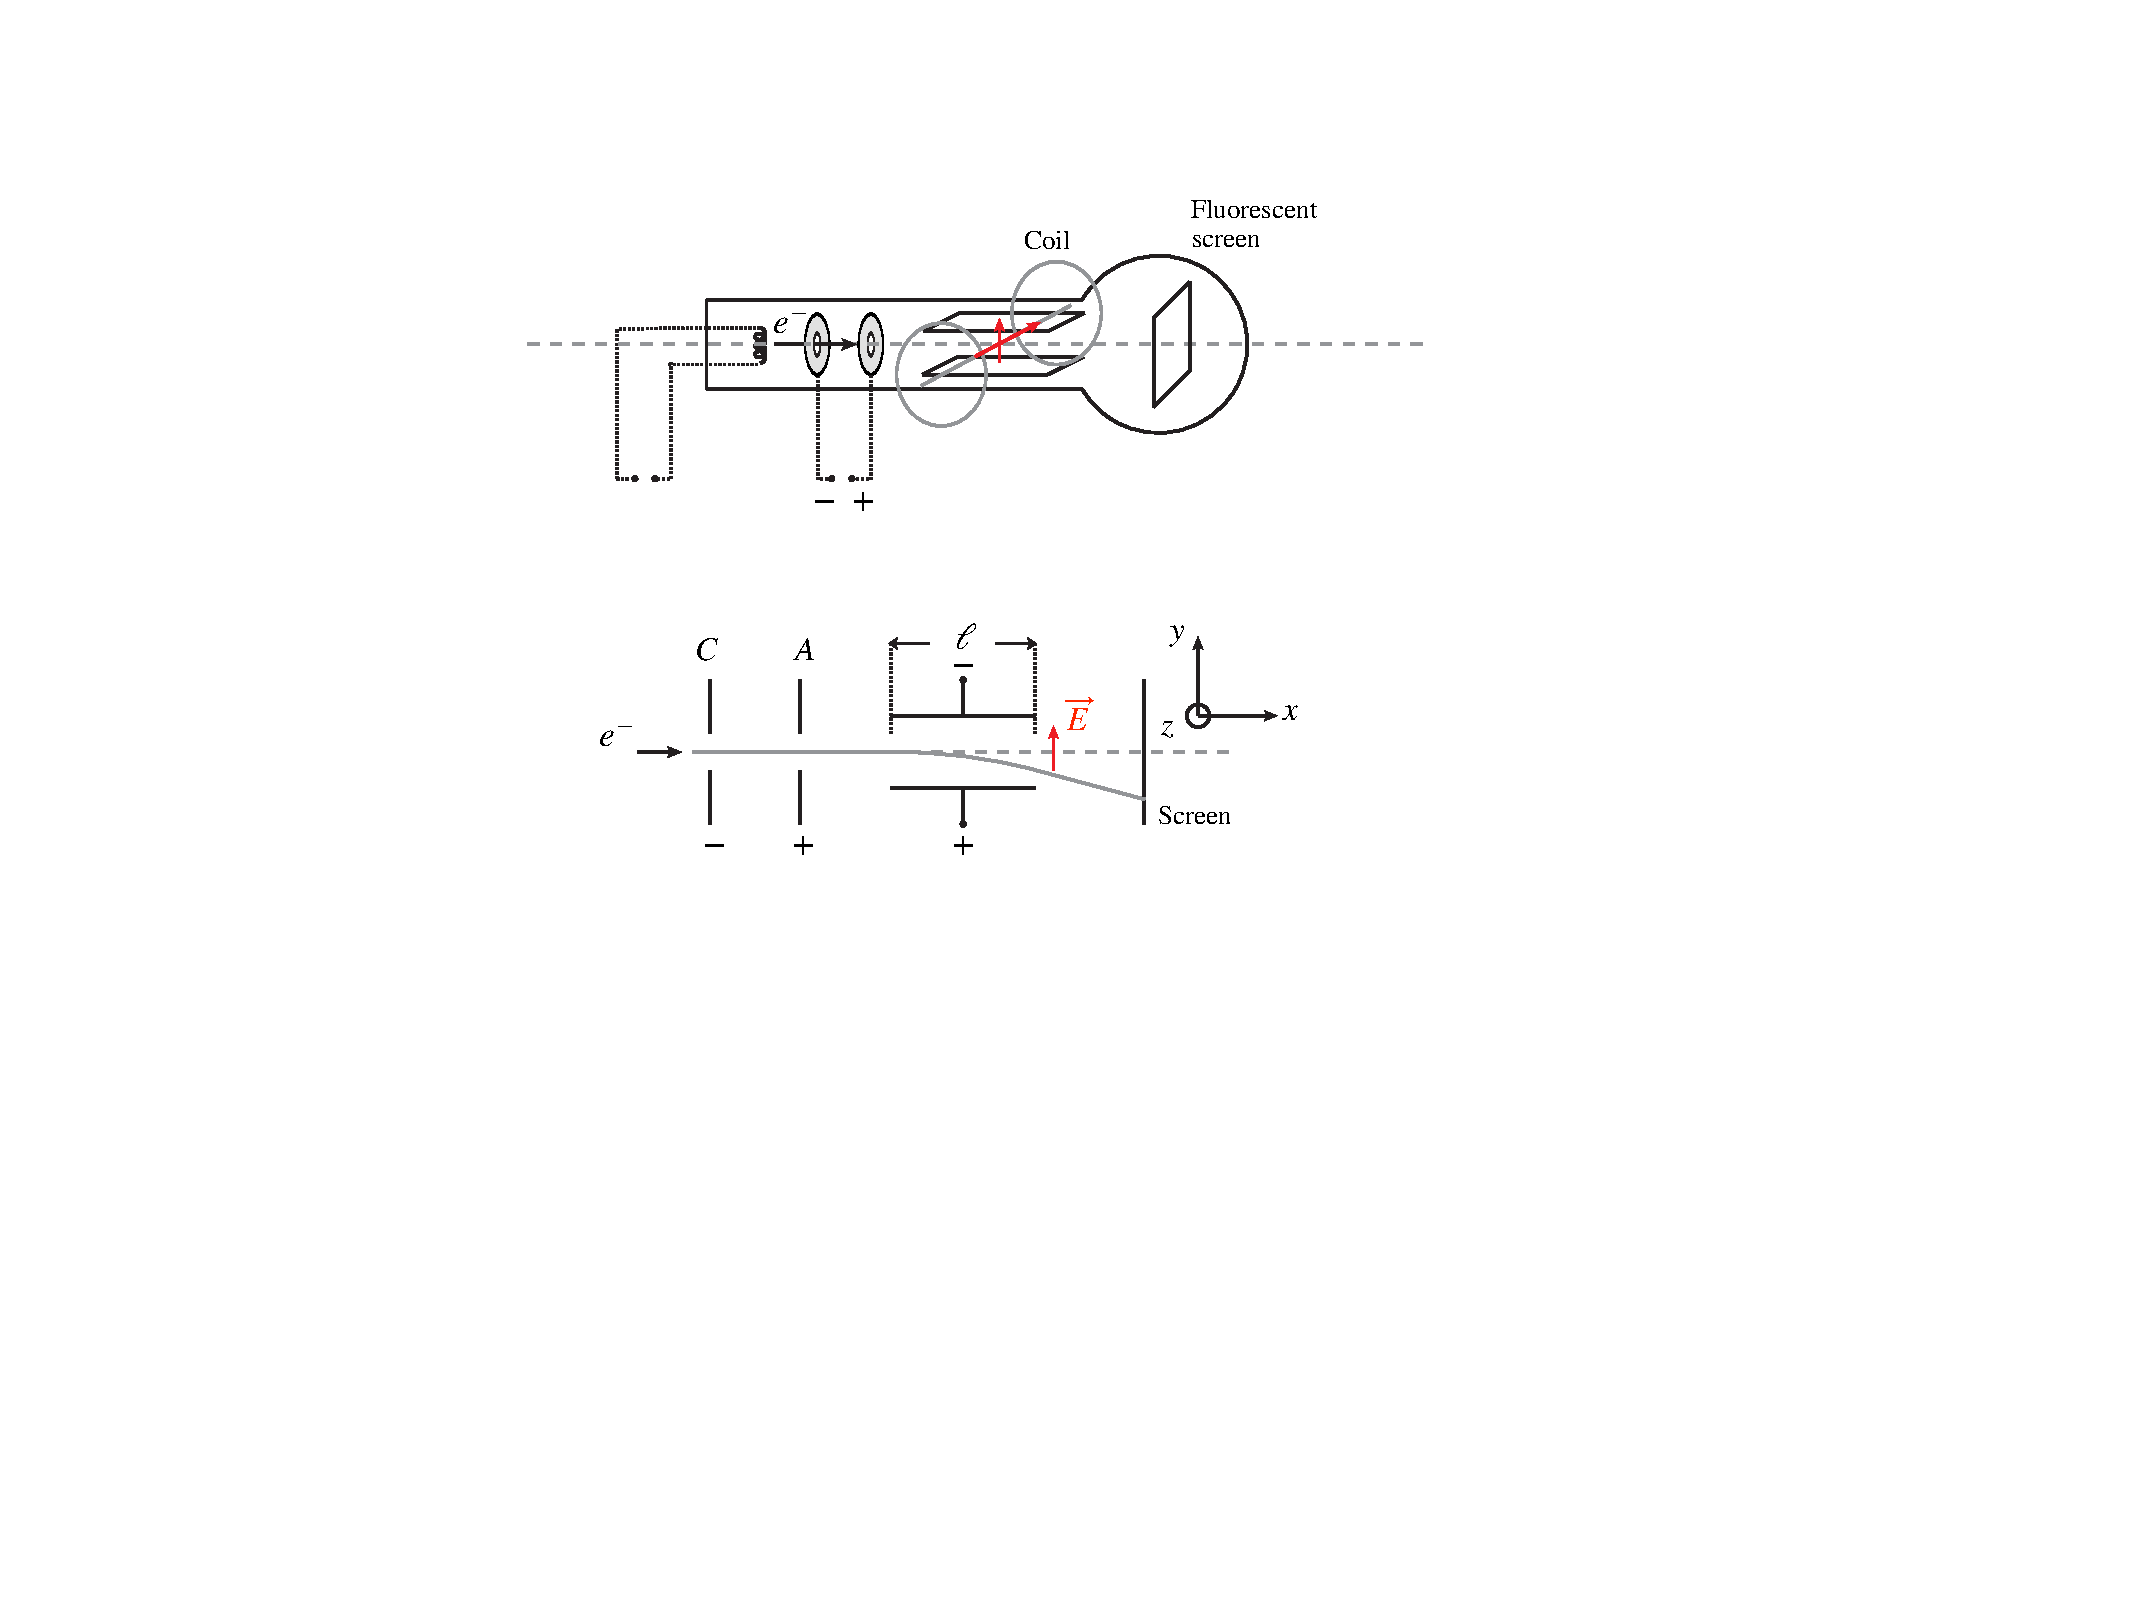
\includegraphics[width=.9\textwidth]{FNSN-Figure-1}

Once accelerated to a velocity $\vec{v} = (v_x, 0, 0)$, the beam passes through two horizontal plates generating an electric field $E$ along the $y$ direction, and coils producing a magnetic field $\vec{B}$ along the $z$ direction. The distance covered by the cathode ray between the plates is $\ell$, and the time passed through the plates is $\Delta t$ where:

$$ v_x = \frac{\ell}{\Delta t}.$$

In the presence of only the electric or only the magnetic field, the cathode rays are bent in the $y$ direction, thus showing that cathode rays are charged particles. The expected deviation of the rays can be computed assuming they are made of particles of mass $m$ and charge $q$: if we write $\vec{F} = q \vec{E} = m \vec{a}$, then

\begin{equation*} m \frac{dv}{dt} = q E \; \; \Rightarrow \; \; v = \int_0^{\Delta t} q \frac{E}{m} dt = q\frac{E}{m}\Delta t,\end{equation*}

and the vertical displacement can then be computed simply as

\begin{equation*}\Delta y = \int_0^{\Delta t} v dt  = \frac{1}{2}  q\frac{E}{m} \Delta t^2 = \frac{1}{2} q \frac{E}{m} \frac{\ell^2}{v_x^2} \end{equation*}

In order to determine the unknown $v_x$,  Thomson had the idea to apply a magnetic field $\vec{B}$ which could be controlled by the currents in the coils. The resulting force exerted on the cathode ray can then be expressed as

\begin{equation*}\vec{F} = q (\vec{E} + \vec{v} \wedge \vec{B}).\end{equation*}

Assuming that the region immersed in the magnetic field is the same as that covered by the electric field, varying the magnetic field in order to compensate perfectly the deviation of the electric field will then yield a measurement of the velocity $v_x$:

\begin{equation*} \vec{F} = \vec{0} \; \; \Rightarrow \; \; q(E - v_x . B) = 0,\end{equation*}

which yields the $v_x=\frac{B}{E}$.

From the measurement without the magnetic field, which yields $\Delta y$, and the measurement of the magnetic field needed to compensate the effect of the electric field, $B$, one can obtain a measurement of the ratio $q/m$:

$$ \frac{q}{m} = 2 \Delta y \frac{E}{\ell^2 B^2} $$

Thompson verified that $q/m$ did not depend neither on the gas in the tube, nor on the cathode material chosen. He therefore established the existence of a negatively charged particle, the electron.
    \end{experiment}    
     \end{framed}       

In his study of the deflection of the cathode rays under the combined effect of electric and magnetic fields, Thomson demonstrated that not only they were associated to negative electric charges: they were also made of particles with a definite relation between charge and mass. The denomination "electrons" was proposed by G. J. Stoneyin 1891 to describe these particles.\\

It is interesting to note that the charge to mass ratio for the cathode rays is much larger than the ratio of the elementary charge divided by the elementary mass, as determined in the case of Faraday's electrolysis experiments. This showed that there seem to be two types of components in the atom, with very different masses or very different charges. Assuming that the charges are the same (since the atom is electrically neutral, there had to be charges that mutually balance), the mass of the electrons had to be much lighter.\\

\section{The Zeeman effect}

Interestingly, during the same period as Thomson's discovery another striking discovery was made on a completely different subject: the impact of a magnetic field on the  emission of light. First intuitions on a possible effect were formulated by Faraday, but it wasn't until the works of Pieter Zeeman in 1896 that the effect was observed. Zeeman demonstrated that in the presence of a magnetic field the spectral lines of a light source show different components. This effect was first observed right before the discovery of the electron, and it allows to independently evaluate the charge-mass ratio $q/m$ of electrons. \\

The Zeeman effect can be described in a semi-classic fashion starting from the Bohr model of the atom, which will be described in more detail in Chapter~\ref{chap:InteractionsInMatter}. Considering a circular orbit of electrons with quantized angular momentum, for an electron with a velocity $v$ the electric current in the loop of the orbit of the electron will be given by

\begin{equation*} I = -\frac{e}{T}=-e \frac{v}{2 \pi r}, \end{equation*}
where $T$ is the period of the orbit and $r$ its radius.

\begin{figure}
  \centering
  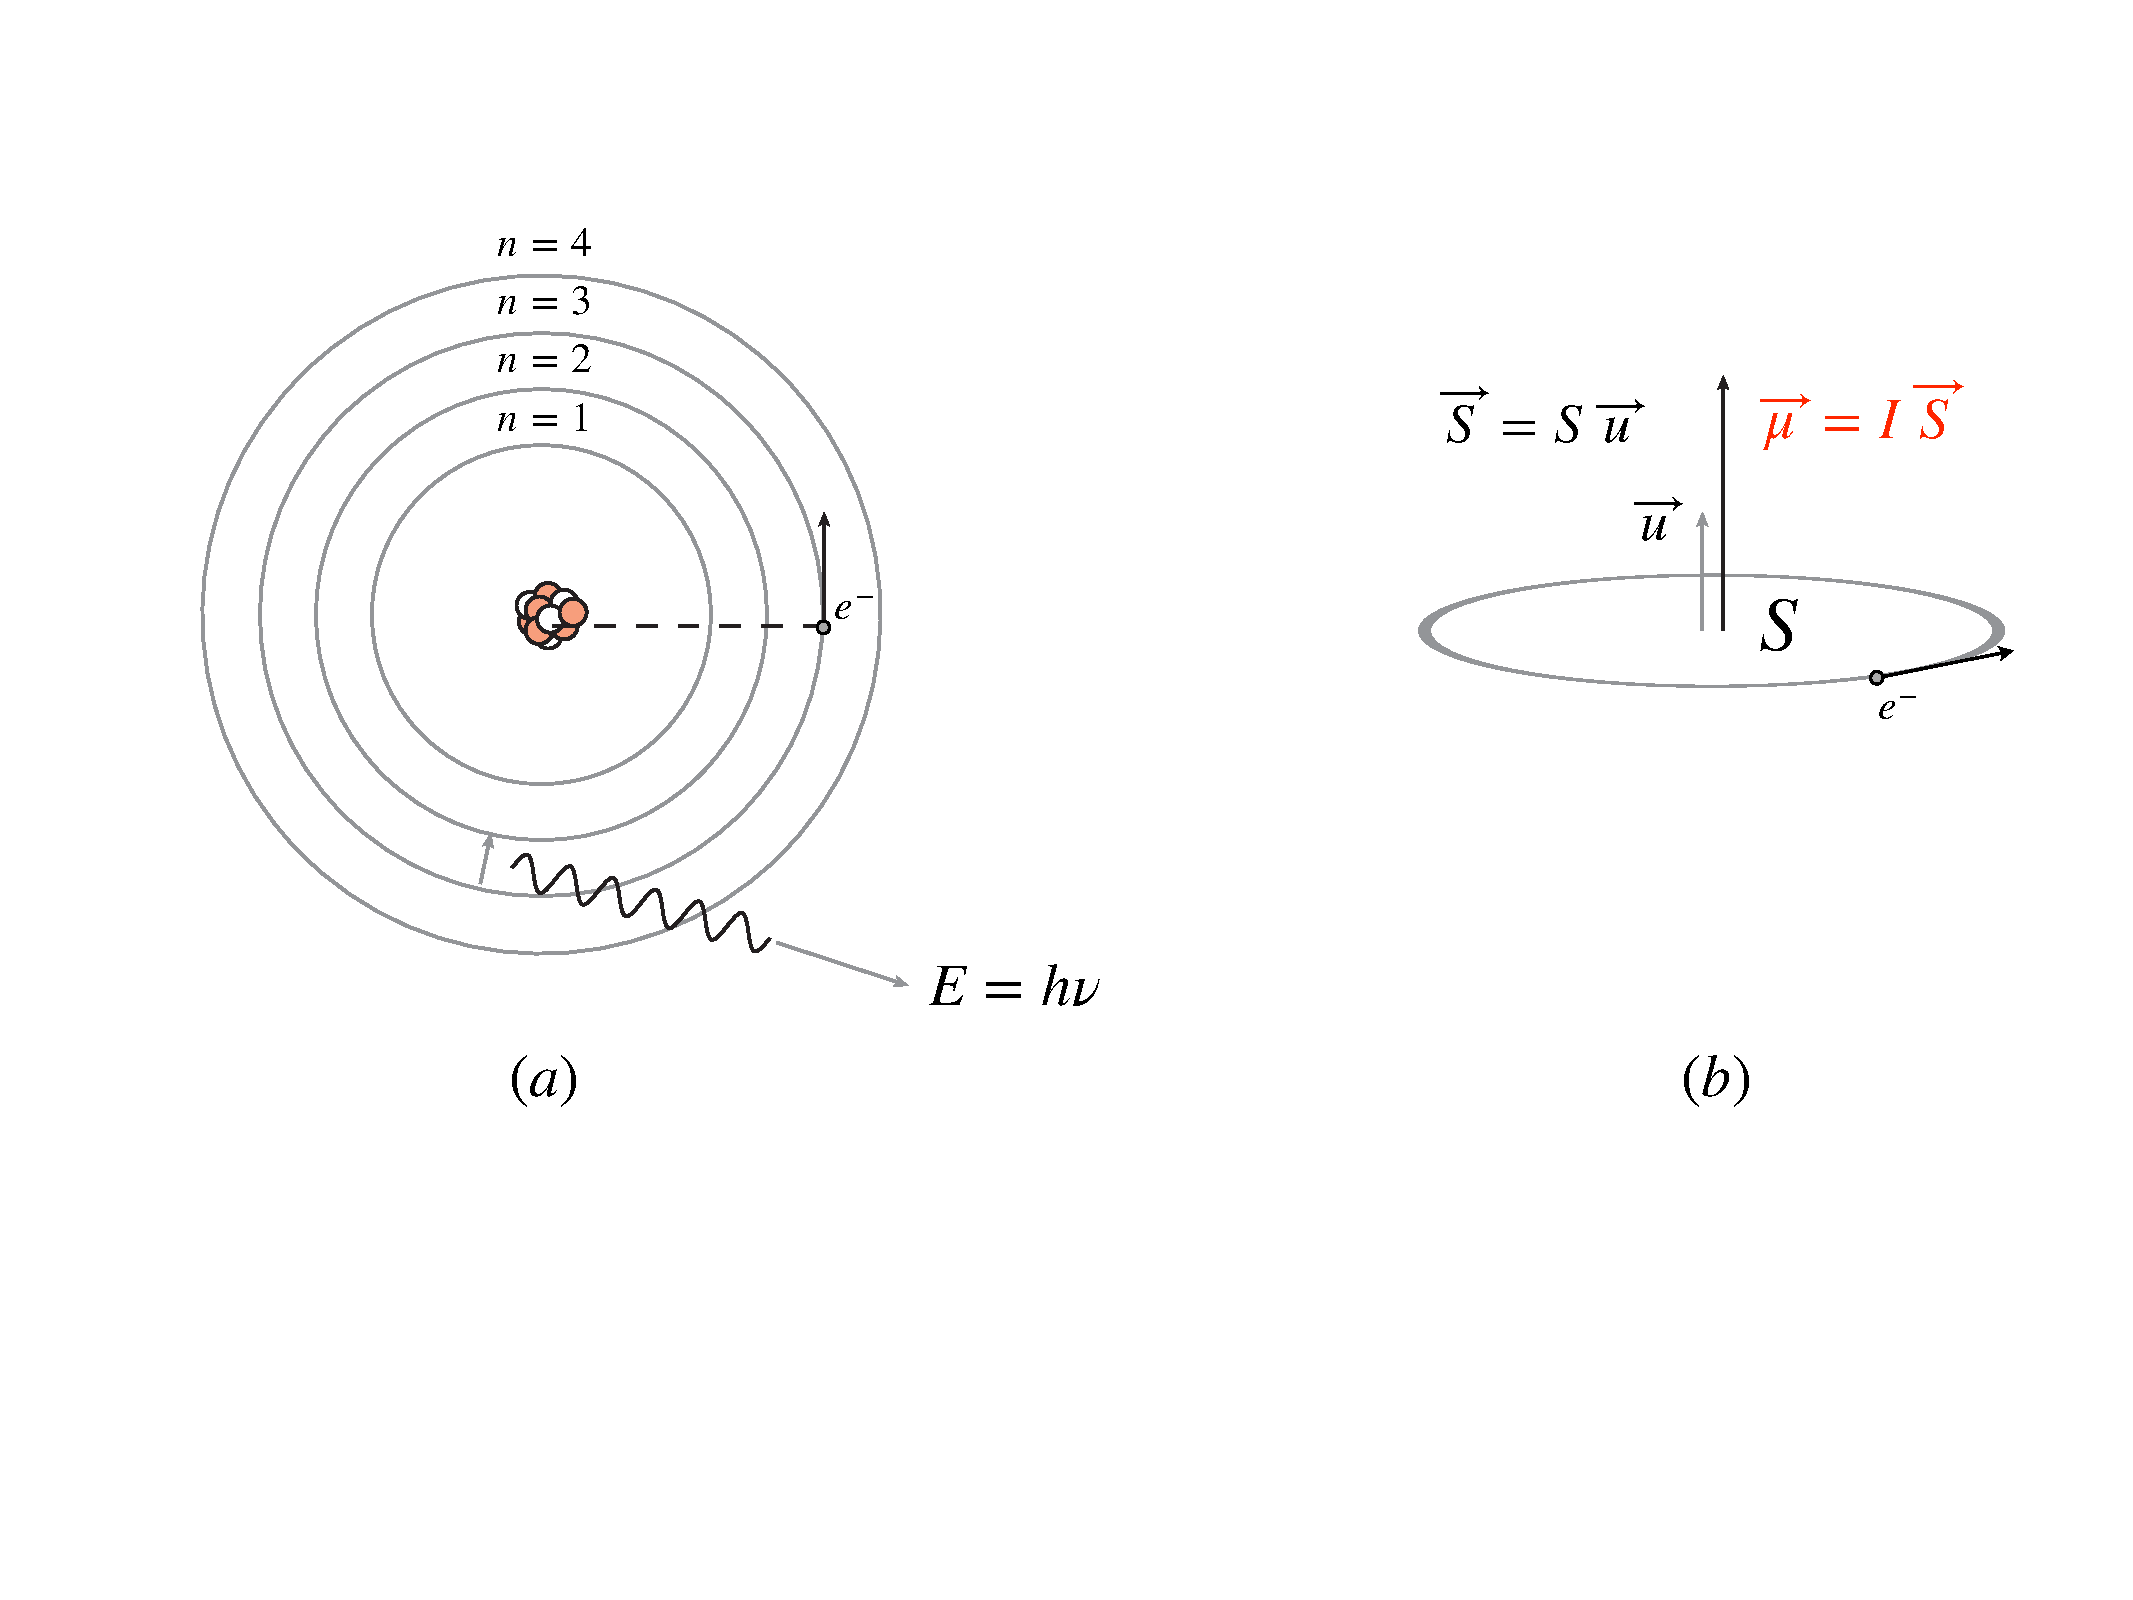
\includegraphics[width=0.8\textwidth]{Bohr}
\caption{Illustration of (a) the Bohr atomic model and (b) the magnetic moment created by the circular orbit of the electron.}  \label{fig:Bohr}
\end{figure}{}
 

The electric current of the orbit creates a magnetic moment (see Fig.~\ref{fig:Bohr}) $\vec{\mu}$:

\begin{equation*} \vec{\mu} = I \, \vec{S} = -e v \frac{r}{2} \vec{u}, \end{equation*}
where $S=\pi r^2$ is the surface of the circular orbit, and $\vec{u}$ the unit vector normal to this surface. The magnetic moment can then also be expressed in terms of angular momentum as:
\begin{equation*} \vec{\mu} = -\frac{e}{2 m_e} \vec{L}, \end{equation*}
where $\vec{L} = \vec{r} \wedge \vec{p} = m_e vr \vec{u}$ is the  angular momentum of the electron, and $m_e$ its mass. The quantization of the angular momentum is obtained by resolving the Schr\"odinger equation for the hydrogen atom: the eigenvalues of the operator $L^2$ are
\begin{equation*}L^2 = \ell (\ell +1) \hslash^2,\end{equation*}
where $\ell$ is the orbital quantum number.

If the atom is immersed in a magnetic field $\vec{B}$, the potential energy of the system will be given by
\begin{equation*} E = \vec{\mu} \cdot \vec{B} = \frac{e}{2 m_e} \vec{L} \cdot \vec{B}, \end{equation*}
where in the Bohr model the projections of $\vec{\ell}$ along the $z$ direction\footnote{Of course, the choice of the direction $z$ is arbitrary.} are $\ell_z = m_{\ell} \cdot \hslash$, where $m_{\ell}$ can take the values:
\begin{equation*} m_{\ell} \in \{ -\ell, -\ell+1, \dots \ell+1, \ell \}.\end{equation*}
In this case the orbitals are not degenerate anymore, but they are rather split. The magnitude of the splitting will yield a difference in energy (with respect to the degenerate line) of:
\begin{equation*} \Delta E = \frac{e}{2 m_e}m_{\ell} \hslash B = \mu_B m_{\ell} B,\end{equation*}
\noindent where $\mu_B = \frac{e \hslash}{2 m_e}$ is called \emph{Bohr magneton}, and depends on the ratio $e/m_e$.

By measuring displacement of spectral lines $\Delta E$ induced by the presence of the magnetic field, one can therefore measure the ratio between the charge and mass of the electron. Zeeman found the same value as in the case of the Thomson experiment:

$$ \frac{e}{m} \sim 1.76 \cdot 10^{11} C (Kg^{-1})$$

It is interesting to note that well before the discovery of the structure of atoms and the existence of nuclei, Zeeman demonstrated an effect, that would prove extremely important in probing the atomic model, once the theoretical understanding of the atom would have progressed sufficiently to describe it quantitatively.  \\

\section{The Millikan experiment and the Charge of the Electron}

The measurement of the charge -- and consequently the mass -- of the electron came later, with a very original experiment by Robert Millikan, in 1907. His experiment was based on  the study of fine oil droplets moving in air. The small drops were either charged by friction on the spout of the atomizer, or by using a X ray source.\\

\begin{figure}
    \centering
      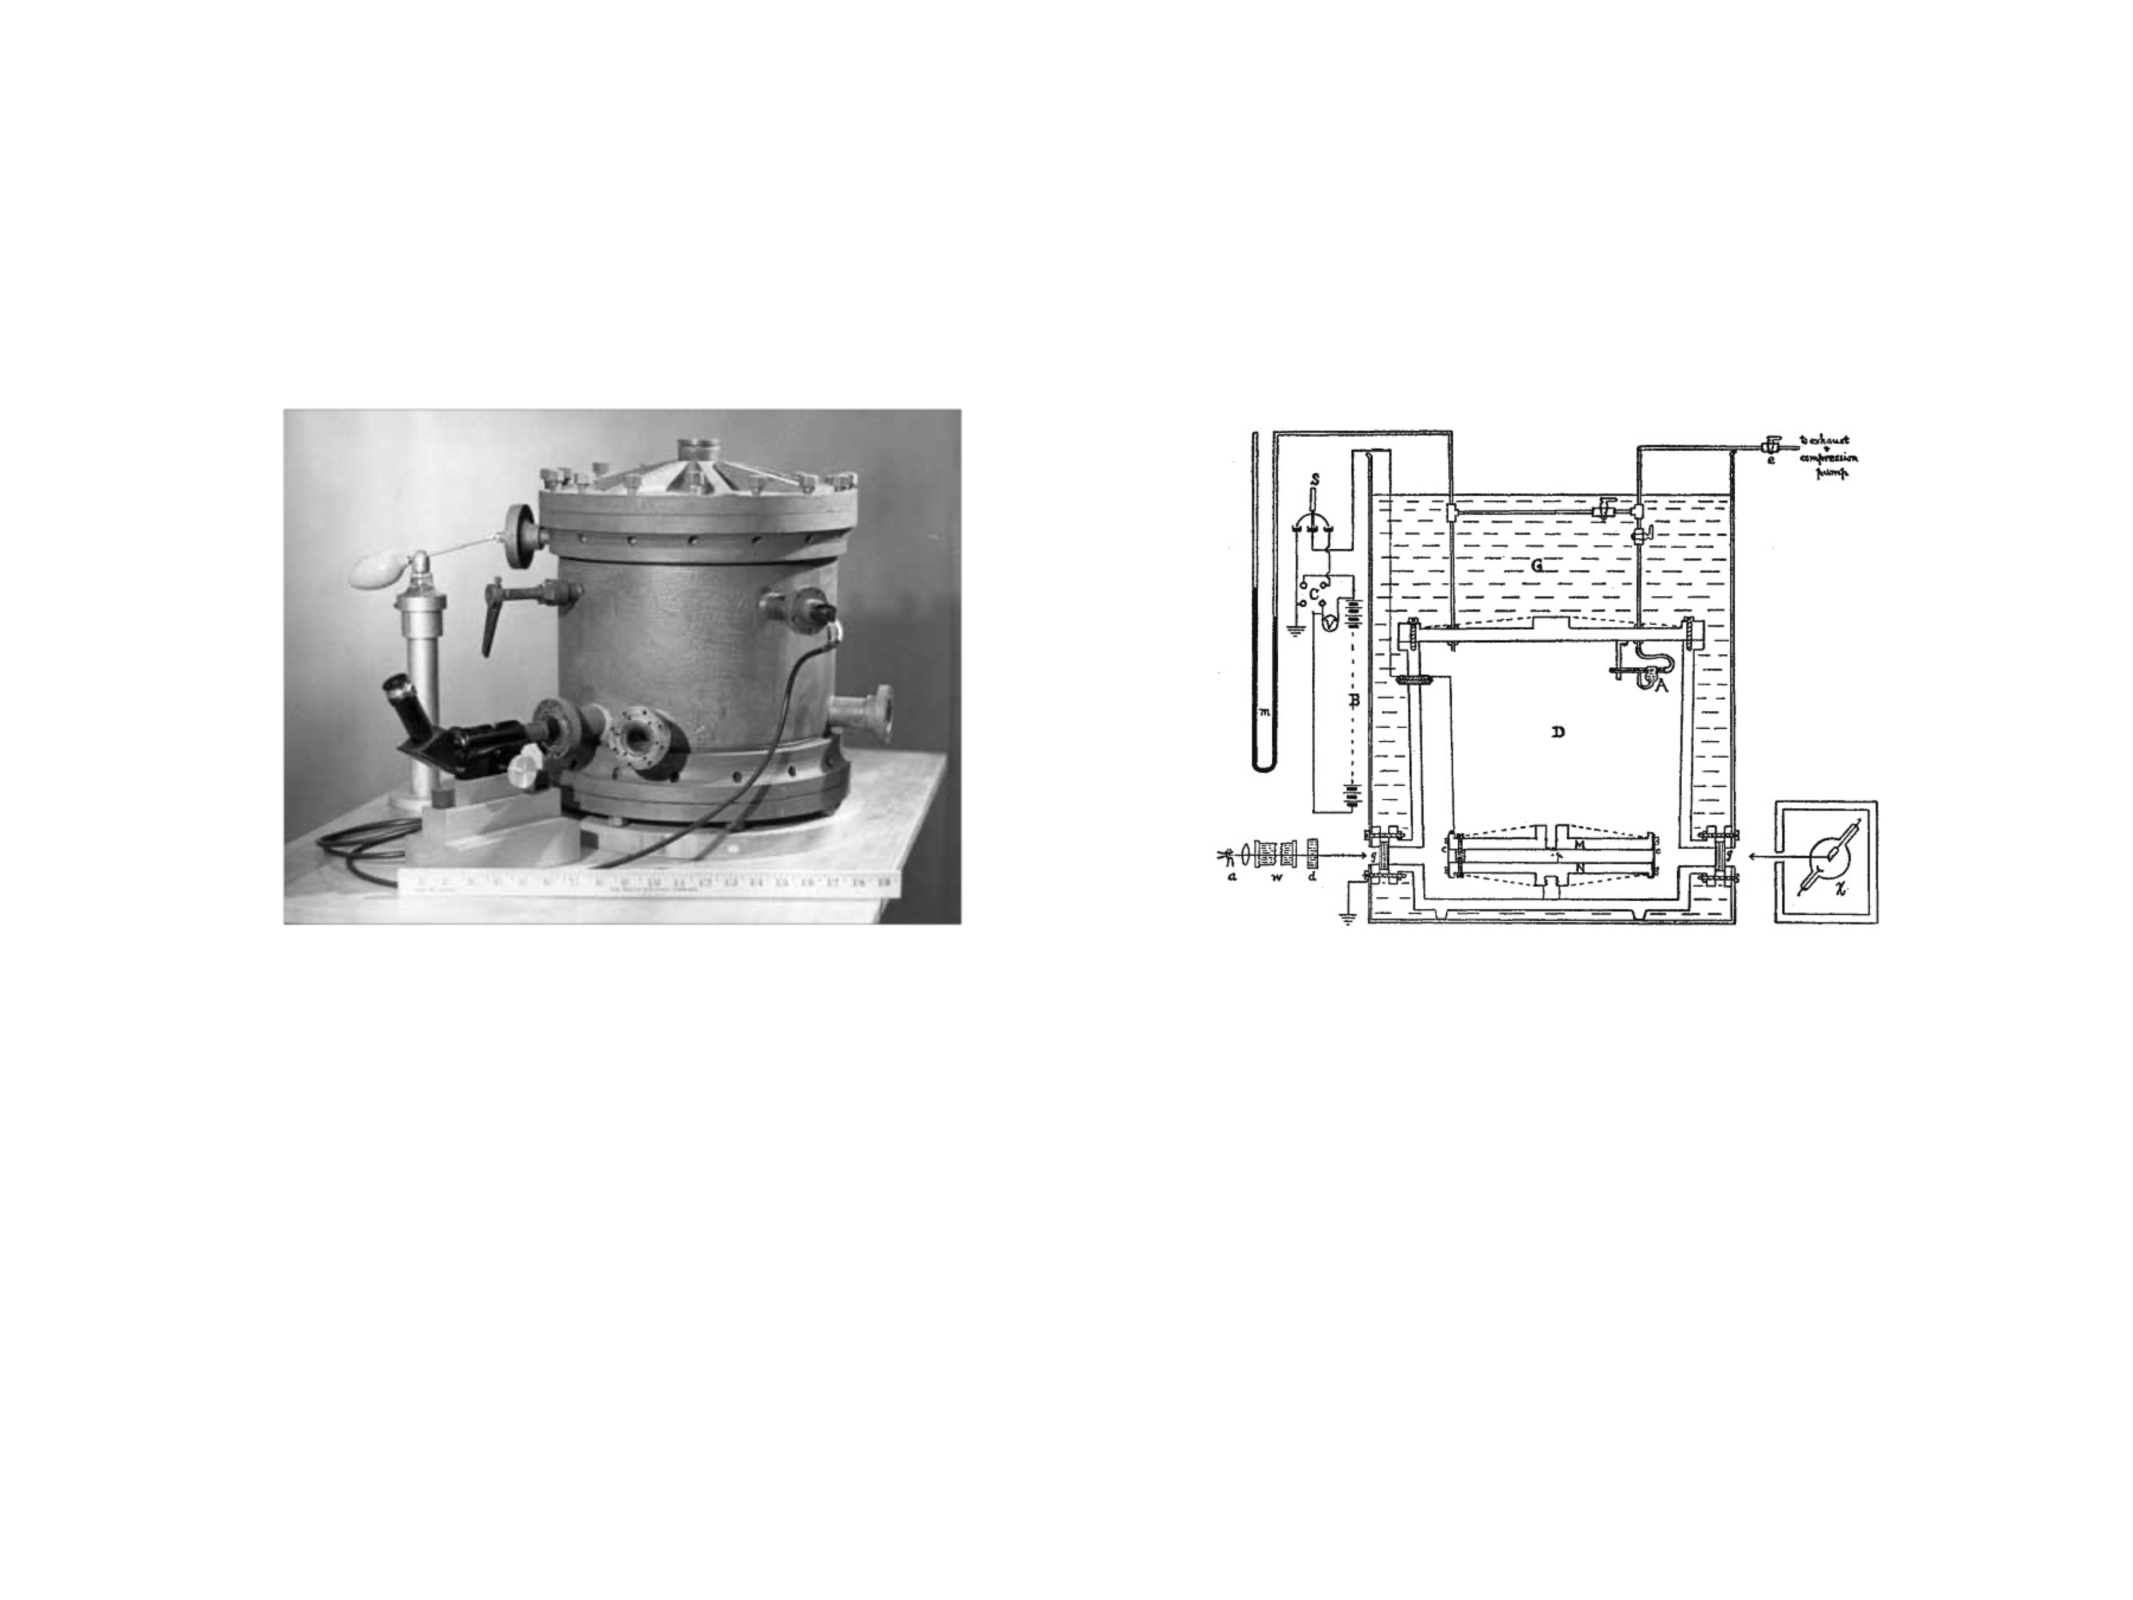
\includegraphics[width=1.0\textwidth]{Millikan}
    \caption{The Millikan experiment setup (left) and a schematic view from the original article (right). M and N represent the condenser plates, A designates the atomizer and in X the "R\"ontgen" (X ray) source is placed. The brass Vessel D is immersed in a gas-engine oil bath at constant temperature with fluctuations not larger than \SI{0.2}{\deg}.}
    \label{fig:Millikan}
\end{figure}

The setup of the experiment is illustrated in Fig.~\ref{fig:Millikan}. The movement of the spheric body in a fluid is subject to a frictional force proportional to the velocity ($v_0$) and to the radius ($r$) of the moving body. This is expressed by Stoke's law,
\begin{equation*}
     F = 6 \pi \eta r v_0,
\end{equation*}
where $\eta$ is the viscosity of the medium in which the body is moving. If we call the density of the moving body $\rho$, and consider that a droplet is -- to a good approximation -- a sphere, then its mass can be expressed in the following way:
\begin{equation*}M = \frac{4}{3} \pi r^3 \rho,\end{equation*}
where $\rho$ is the oil density. \\

The resultant buoyancy of the sphere due to Archimedes' principle in air, corresponding to the mass of air displaced by the volume of the droplet, is
\begin{equation*}M_a = \frac{4}{3} \pi r^3 \rho_a\end{equation*}
where $\rho_a$ is the density of air. Therefore, when the droplet reaches a uniform speed, all forces cancel yielding:
\[
\frac{4}{3} \pi r^3 (\rho-\rho_a) g = 6 \pi \eta r v_0.
\]
One can measure the velocity of individual drops by observing their fall through a microscope. Given the above formula, measuring $v_0$ gives the radius of the droplets:

$$ r^2 = \frac{9 \eta v_0}{2 g (\rho - \rho_a)}.$$

By applying an electric field in such a way that the electrostatic force is opposite to gravity, the force $qE$ will slow the fall down. The voltage applied is high enough to generate an electric field of approximately \SI{6000}{V/cm}. The voltage is then tuned in order to stop the motion of the droplets ($v = 0$), i.e.

$$ q \frac{V}{d} - Mg = 6 \pi \eta r v = 0.$$

Having previously measured the radius of the droplets was therefore essential to infer the mass of the droplets. This experiment yielded measurements of the elementary charge of the electron to be:
$$ e = 1.59 \cdot 10^{-19} \; \; {\rm C},$$
slightly smaller than the currently known value of $1.6 \cdot 10^{-19}$~C.\\

It is now known that Millikan's value was very slightly biased due to an error in the estimate of the viscosity. This insignificant mistake had a very interesting impact in understanding measurement biases and is often cited as such due to the fact that many subsequent experiments found values close to the one found by Millikan. The experiment is therefore often given as an example of non-conscious bias towards an already measured value. \\

From the measured ratio of $e/m$ the mass of the electron can be determined, yielding

\begin{center}
\fbox{
$m_e = 9.109 \cdot 10^{-31} \; {\rm kg} $,
}
\end{center}
which corresponds to $m_e c^2 = 0.511$~MeV in microscopic units as discussed in Chapter~\ref{chap:units}.


\section*{Take-home lessons}
\begin{itemize}
    \item Ancient atomism was surprisingly visionary in its (merely philosophical) attempt to describe nature. Empirical observations in Chemistry (e.g. Dalton's and Gay-Lussac's laws) built the foundations of modern atomism. Faraday's laws on electrolysis suggested the existence of unit charges and of the concept of elementary particle (then identified as the proton). The existence of atoms was proved later, with the explanation of brownian motion.
    \item Different kinds of radioactivity were discovered, and classified first based on their properties, and then based on our understanding of elementary particles. 
    \item $\beta^+$ radiation, consisting of electrons, was originally observed in the form of cathode rays.
    \item X rays were observed when sending electrons (cathode rays) on atoms: they were later understood to be photons which were either emitted by the electrons due to bremsstrahlung radiation (continuum spectrum due to the deflection of their path by the atomic nucleus), or photons emitted by an atomic electron which moved from an outer to an inner  level to replace another atomic electron kicked off by the cathode ray (discrete spectrum).
    \item Spontaneous emission of radioactivity by materials was later discovered and soon understood to be different from X rays. Radiation was classified as $\alpha$, $\beta$ and $\gamma$ depending on its deflection by magnetic fields. We now know that $\alpha$ particles are Helium nuclei ($^4He^{2+}$), $\beta^-$ radiation is made of electrons, $\beta^+$ of positrons (the electron anti-particle), and $\gamma$ and X rays are made of photons of different typical energies.
    \item Experiments helped measure the basic properties of particles. The electron charge-mass ratio could be measured (i) by altering the path of cathode rays using electric and magnetic fields, or (ii) with a measurement of the splitting of energy levels induced by the presence of magnetic field, as explained by the Zeeman effect in terms of the angular momentum and Bohr magneton of electrons.
    \item The charge of the electron could be measured by first charging small oil droplets (e.g. by friction or irradiation with X rays), and then using an electric field to stop their fall in air. 
\end{itemize}
\section*{Questions}
\begin{itemize}
    \item How many protons are there in a \si{kg} of carbon?
    \item Can you draw the $1s\to2p$ spectral line of hydrogen with and without magnetic field?
\end{itemize}